\documentclass[12pt,a4paper]{article}

% ============================================================
% ПРЕАМБУЛА
% ============================================================

\usepackage{ifxetex}
\ifxetex
    \usepackage{fontspec}
    \usepackage{polyglossia}
    \setdefaultlanguage{russian}
    \setotherlanguage{english}
    \setmainfont{Times New Roman}
    \setsansfont{Helvetica}
    \setmonofont{Courier New}
    \newfontfamily\cyrillicfont{Times New Roman}
    \newfontfamily\cyrillicfontsf{Helvetica}
    \newfontfamily\cyrillicfonttt{Courier New}
\else
    \usepackage[T2A]{fontenc}
    \usepackage[utf8]{inputenc}
    \usepackage[russian]{babel}
    \usepackage{cmap}
    \usepackage{lmodern}
\fi

\usepackage{amsmath, amssymb, amsfonts, amsthm}
\usepackage{geometry}
\usepackage{graphicx}
\usepackage{float}
\usepackage{booktabs}
\usepackage{array}
\usepackage{caption}
\usepackage{titlesec}
\usepackage{xcolor}
\usepackage{microtype}
\usepackage{hyperref}

\geometry{
    left=25mm,
    right=15mm,
    top=20mm,
    bottom=20mm
}

\sloppy

\hypersetup{
    colorlinks=true,
    linkcolor=black,
    urlcolor=blue!60!black,
    citecolor=black
}

\setlength{\parindent}{1.0cm}
\setlength{\parskip}{2pt}

\titleformat{\section}{\normalfont\bfseries\large}{\thesection.}{0.5em}{}
\titleformat{\subsection}{\normalfont\bfseries\normalsize}{\thesubsection.}{0.5em}{}

\titlespacing*{\section}{0pt}{12pt}{4pt}
\titlespacing*{\subsection}{0pt}{8pt}{2pt}

\captionsetup{labelsep=period, justification=centering, font=small}

% ============================================================
% ДОКУМЕНТ
% ============================================================

\begin{document}

% ============================================================
% ТИТУЛЬНЫЙ ЛИСТ
% ============================================================

\begin{titlepage}
    \begin{center}
        \textbf{МИНИСТЕРСТВО НАУКИ И ВЫСШЕГО ОБРАЗОВАНИЯ\\
        РОССИЙСКОЙ ФЕДЕРАЦИИ}\\[0.4cm]

        \textbf{Федеральное государственное автономное образовательное учреждение\\
        высшего образования}\\[0.2cm]

        \textbf{<<Национальный исследовательский университет ИТМО>>}\\[1.2cm]

        \textbf{Факультет технологий искусственного интеллекта}\\[1.5cm]

        \textbf{\Large Лабораторная работа}\\[0.4cm]

        по дисциплине\\
        \textbf{<<Функциональный анализ>>}\\[0.8cm]

        \textbf{\Large Регрессия по функциональным данным:}\\[0.2cm]
        \textbf{\Large линейные функционалы и метрические методы}\\[0.6cm]

        \textbf{Кейсы №4 и №6}\\[1.5cm]
    \end{center}

    \begin{flushright}
        Выполнил:\\
        студент группы J3210\\
        \textbf{Тищенко Павел Валерьевич}
    \end{flushright}

    \vfill

    \begin{center}
        Исходный код: \url{https://github.com/paulhowever/funkan_tischenko_j3210}\\[0.4cm]
        Санкт-Петербург, 2026
    \end{center}
\end{titlepage}

% ============================================================
% 1. ВВЕДЕНИЕ
% ============================================================

\section{Введение}

В прикладных задачах объект наблюдения часто задаётся не вектором, а функцией $x(t)$, $t\in[0,1]$ (временной ряд, сигнал датчика, профиль и т.\,п.). По функции требуется предсказать число $y\in\mathbb{R}$. Прямо учить регрессионную модель на функции нельзя: $L_2[0,1]$ — бесконечномерное гильбертово пространство, а на дискретной сетке $N=320$ точек --- это всё ещё в среднем больше, чем число обучающих объектов. Поэтому функцию сначала надо «сжать» в конечномерный вектор признаков, не теряя существенной структуры.

Работа объединяет два подхода в одну схему:
\[
x(t)\;\xrightarrow{\text{кейс 4}}\;
z=\bigl(\langle x,\varphi_1\rangle,\dots,\langle x,\varphi_m\rangle\bigr)
\;\xrightarrow{\text{кейс 6}}\;\hat y.
\]

\emph{Кейс 4} --- параметрический подход: функция превращается в конечномерный вектор линейных функционалов, на котором обучается линейная (или ridge) регрессия; восстанавливается весовая функция $w(t)$, дающая глобально интерпретируемое предсказание.

\emph{Кейс 6} --- непараметрические метрические методы: ядерная регрессия Надарая--Ватсона с фиксированным и переменным окном, а также робастная схема LOWESS. Эти методы применены и к признакам кейса 4, и к двум табличным датасетам --- \textit{Diabetes} и \textit{California Housing}, чтобы оценить общность подхода на стандартных регрессионных задачах.

% ============================================================
% 2. ДАННЫЕ
% ============================================================

\section{Данные}

\textbf{Синтетические функциональные данные:}
\[
x_i(t)=a_i\sin(2\pi t)+b_i\cos(2\pi t)+c_i t+\varepsilon_i(t),\qquad
y_i=2\!\int_0^1\!x_i(t)\sin(2\pi t)\,dt-\!\int_0^1\!x_i(t)t\,dt+\eta_i.
\]
Истинная зависимость линейна по интегральным функционалам, шум функции $\varepsilon_i$ и шум ответа $\eta_i$ --- нормальные. Такая конструкция выбрана специально: она позволяет проверить, насколько хорошо разные системы функционалов восстанавливают истинную весовую функцию $w(t)=2\sin(2\pi t)-t$.

\textbf{Реальные датасеты:} \textit{Diabetes} (sklearn, $n=442$, 10 признаков, целевая --- индекс прогрессирования заболевания через год после базовых измерений) и \textit{California Housing} (под-выборка $n=3000$ из $20640$, 8 признаков, медианная цена дома в \$$10^5$). Признаки стандартизуются на обучающей части (z-score). Это критично для метрических методов: иначе компонента с большим масштабом доминирует в евклидовом расстоянии, и модель фактически смотрит только на одну переменную.

\begin{figure}[H]
    \centering
    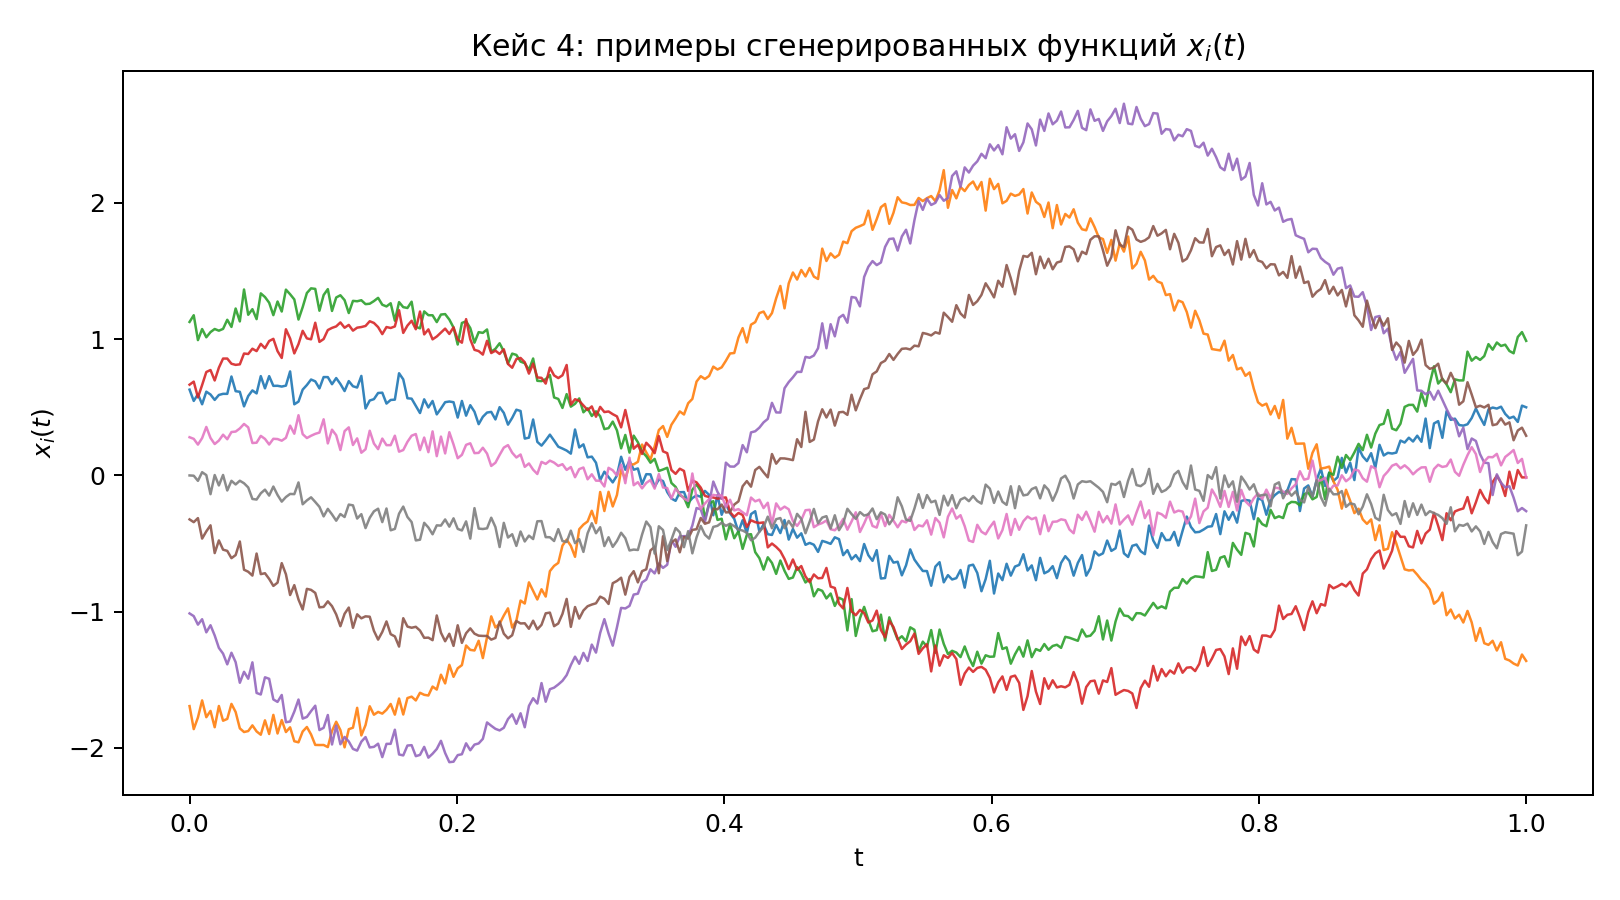
\includegraphics[width=0.78\textwidth]{report_outputs/figures/sample_functions.png}
    \caption{Примеры сгенерированных функциональных данных $x_i(t)$.}
    \label{fig:sample_functions}
\end{figure}

% ============================================================
% 3. ЛИНЕЙНЫЕ ФУНКЦИОНАЛЫ
% ============================================================

\section{Кейс 4. Линейные функционалы и регрессия}

\subsection{Функционалы интегрального вида в $L_2[0,1]$}

Линейным функционалом называется отображение $L\colon L_2[0,1]\to\mathbb{R}$, удовлетворяющее $L(\alpha x+\beta y)=\alpha L(x)+\beta L(y)$. Согласно теореме Рисса о представлении, любой непрерывный линейный функционал в гильбертовом пространстве $L_2[0,1]$ имеет вид скалярного произведения с некоторым фиксированным элементом этого же пространства:
\[
L_\varphi(x)=\langle x,\varphi\rangle=\int_0^1 x(t)\varphi(t)\,dt.
\]
Функция $\varphi(t)$ играет роль <<шаблона>>: значение $L_\varphi(x)$ показывает, насколько $x(t)$ согласована с $\varphi(t)$. Линейность сразу следует из линейности интеграла:
\[
L_\varphi(\alpha x+\beta y)=\int(\alpha x+\beta y)\varphi\,dt
=\alpha\int x\varphi\,dt+\beta\int y\varphi\,dt=\alpha L_\varphi(x)+\beta L_\varphi(y).
\]
Численная проверка для конкретной пары функционалов на одной из синтетических функций даёт $|L_\varphi(\alpha x+\beta y)-\alpha L_\varphi(x)-\beta L_\varphi(y)|\sim 10^{-9}$, что подтверждает корректность реализации (детали --- в \texttt{tables/linearity\_check.csv}).

Каждой функции $x_i(t)$ ставится в соответствие конечномерный вектор:
\[
z_i=(z_{i1},\dots,z_{im}),\qquad z_{ik}=\langle x_i,\varphi_k\rangle.
\]
Сравниваются три системы функционалов:
\begin{itemize}\setlength\itemsep{0pt}
    \item \textbf{индикаторы подотрезков} $\varphi_k=\mathbf{1}_{[\tau_{k-1},\tau_k]}$ --- локальные средние значения функции на конкретном участке;
    \item \textbf{полиномы} $1,t,t^2,\dots,t^{m-1}$ --- гладкие тренды (моменты функции);
    \item \textbf{тригонометрический базис} $1,\sin(2\pi t),\cos(2\pi t),\sin(4\pi t),\dots$ --- амплитуды периодических компонент (короткий ряд Фурье).
\end{itemize}

\subsection{Численное вычисление интегралов}

Поскольку функции хранятся не аналитически, а на равномерной сетке $\{t_j\}_{j=0}^{N-1}$ с шагом $\Delta t$, скалярные произведения вычисляются по формуле трапеций:
\[
\int_0^1 x(t)\varphi_k(t)\,dt
\approx
\sum_{j=0}^{N-2}\frac{x(t_j)\varphi_k(t_j)+x(t_{j+1})\varphi_k(t_{j+1})}{2}\,\Delta t.
\]
Ошибка квадратуры имеет порядок $O(\Delta t^2)$ для гладких подынтегральных выражений; при $N=320$ это $\sim 10^{-5}$, что заведомо меньше дисперсии шума $\eta_i$ и поэтому не вносит систематического смещения в признаки.

\subsection{Линейная регрессия и нормальные уравнения}

После сборки матрицы признаков $Z\in\mathbb{R}^{n\times m}$ и расширения её столбцом единиц до $X=[\mathbf{1}\,|\,Z]$ модель имеет вид $\hat y=X\beta$. Метод наименьших квадратов минимизирует
\[
Q(\beta)=\|y-X\beta\|^2=(y-X\beta)^T(y-X\beta).
\]
Градиент по $\beta$ равен $\nabla Q=-2X^T(y-X\beta)$. Приравнивая нулю, получаем нормальные уравнения
\[
X^TX\,\hat\beta=X^Ty.
\]
Гессиан $\nabla^2 Q=2X^TX$ положительно полуопределён (а при полном столбцовом ранге $X$ --- положительно определён), поэтому $\hat\beta=(X^TX)^{-1}X^Ty$ --- глобальный минимум.

\subsection{Ridge-регуляризация}

При большом $m$ или сильной зависимости функционалов матрица $X^TX$ становится плохо обусловленной, и оценки $\hat\beta$ начинают сильно колебаться от выборки к выборке. Ridge добавляет к функционалу штраф $\lambda\|\beta\|^2$ ($\lambda\ge 0$):
\[
Q_\lambda(\beta)=\|y-X\beta\|^2+\lambda\|\beta\|^2.
\]
Соответствующие нормальные уравнения
$(X^TX+\lambda I)\hat\beta_\lambda=X^Ty$
дают замкнутое решение
\[
\hat\beta_\lambda=(X^TX+\lambda I)^{-1}X^Ty.
\]
Матрица $X^TX+\lambda I$ всегда положительно определена при $\lambda>0$, поэтому решение существует и единственно даже при сингулярном $X^TX$. Геометрически ridge сдвигает все собственные числа $X^TX$ на $\lambda$, что подавляет направления с малой собственной информативностью.

В терминах bias--variance: МНК-оценка несмещённая, но при плохой обусловленности её дисперсия растёт пропорционально $1/\lambda_{\min}(X^TX)$. Ridge вносит небольшое смещение $\sim\lambda$, но уменьшает дисперсию на порядок большую величину; при правильно подобранном $\lambda$ суммарная MSE предсказания меньше, чем у обычного МНК. Это частный случай теоремы Джеймса--Стейна: в размерности $\ge 3$ можно построить оценку, доминирующую несмещённую МНК-оценку по MSE.

\subsection{Восстановление весовой функции}

Линейная модель имеет вид
\[
\hat y(x)=\beta_0+\sum_{k=1}^{m}\beta_k\langle x,\varphi_k\rangle.
\]
Введём
$w(t)=\sum_{k=1}^{m}\beta_k\varphi_k(t)$. По линейности скалярного произведения:
\[
\langle x,w\rangle
=\Bigl\langle x,\textstyle\sum_k\beta_k\varphi_k\Bigr\rangle
=\sum_k\beta_k\langle x,\varphi_k\rangle,
\]
поэтому $\hat y(x)=\beta_0+\langle x,w\rangle$. Таким образом, бесконечномерная задача регрессии сведена к скалярному произведению с одной фиксированной функцией $w(t)$ --- это даёт прямую интерпретацию: участки $t$, где $|w(t)|$ велико, сильнее всего влияют на прогноз.

\begin{figure}[H]
    \centering
    \begin{minipage}{0.49\textwidth}
        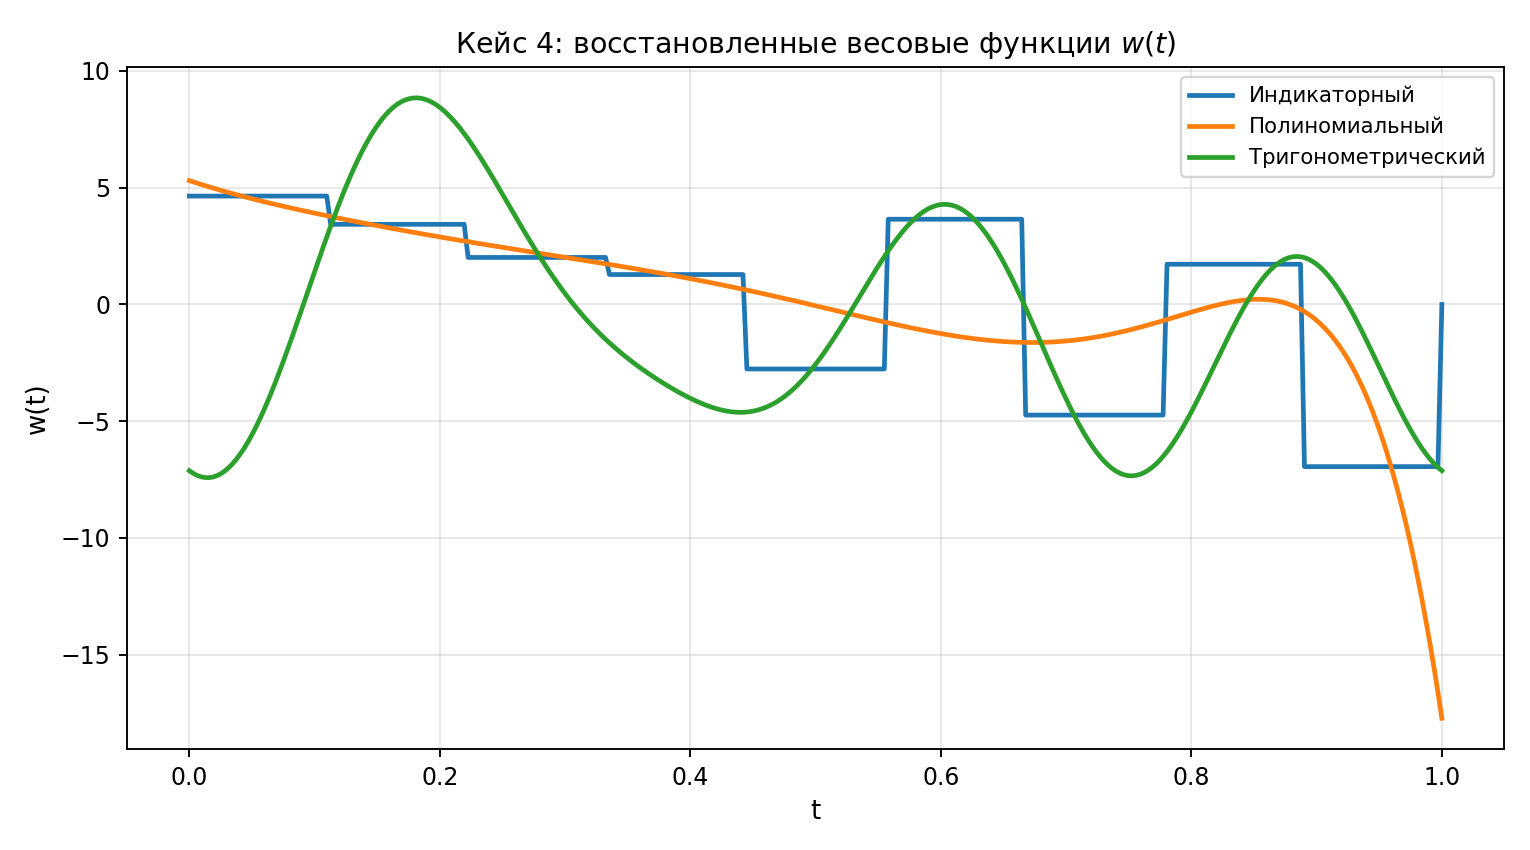
\includegraphics[width=\linewidth]{report_outputs/figures/weight_functions_comparison.png}
    \end{minipage}\hfill
    \begin{minipage}{0.49\textwidth}
        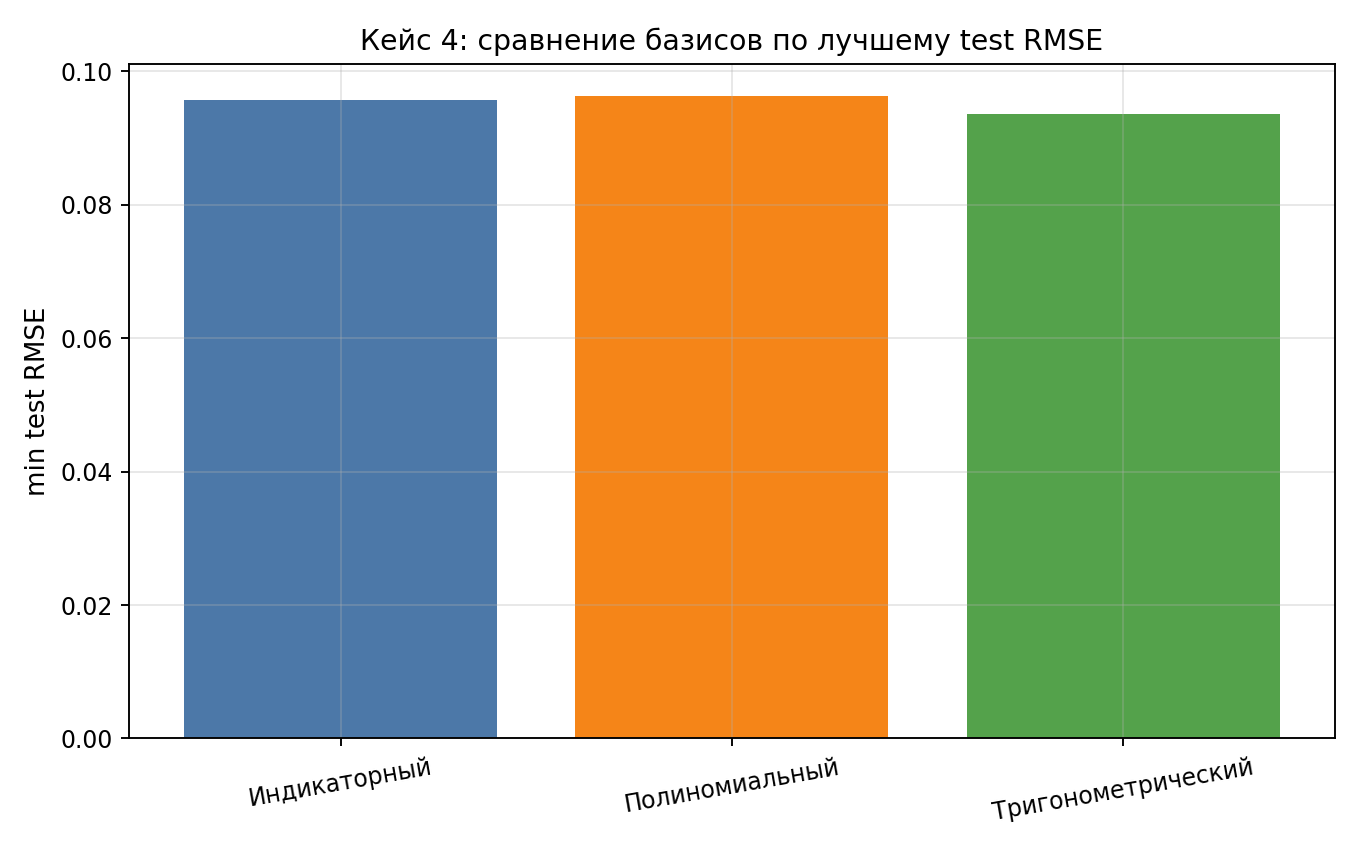
\includegraphics[width=\linewidth]{report_outputs/figures/basis_comparison_rmse.png}
    \end{minipage}
    \caption{Слева: восстановленные $w(t)$ для трёх базисов. Справа: лучший test RMSE по каждому базису.}
    \label{fig:case4_basis}
\end{figure}

\subsection{Эксперименты}

Метрики качества:
\[
\mathrm{MAE}=\tfrac{1}{n}\textstyle\sum_i|y_i-\hat y_i|,\quad
\mathrm{MSE}=\tfrac{1}{n}\textstyle\sum_i(y_i-\hat y_i)^2,\quad
\mathrm{RMSE}=\sqrt{\mathrm{MSE}},\quad
R^2=1-\tfrac{\mathrm{SS}_{\mathrm{res}}}{\mathrm{SS}_{\mathrm{tot}}}.
\]
$\mathrm{MAE}$ устойчива к выбросам, $\mathrm{RMSE}$ сильнее штрафует большие ошибки (соответствует гауссовскому шуму), $R^2$ показывает долю объяснённой дисперсии и удобен для сравнения моделей в разных шкалах. Train/test разделяются как 75/25 случайной перестановкой объектов.

\begin{figure}[H]
    \centering
    \begin{minipage}{0.49\textwidth}
        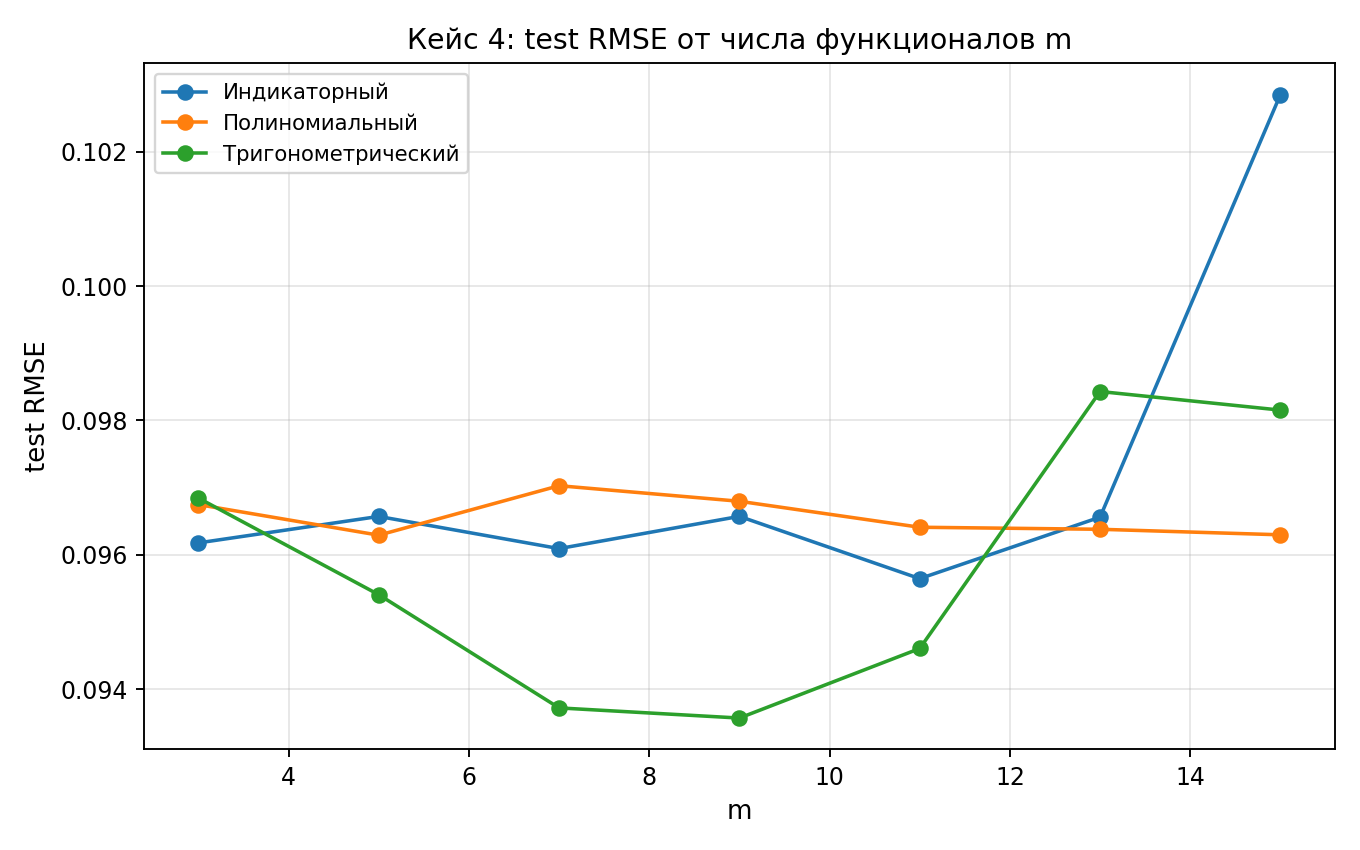
\includegraphics[width=\linewidth]{report_outputs/figures/rmse_vs_m.png}
    \end{minipage}\hfill
    \begin{minipage}{0.49\textwidth}
        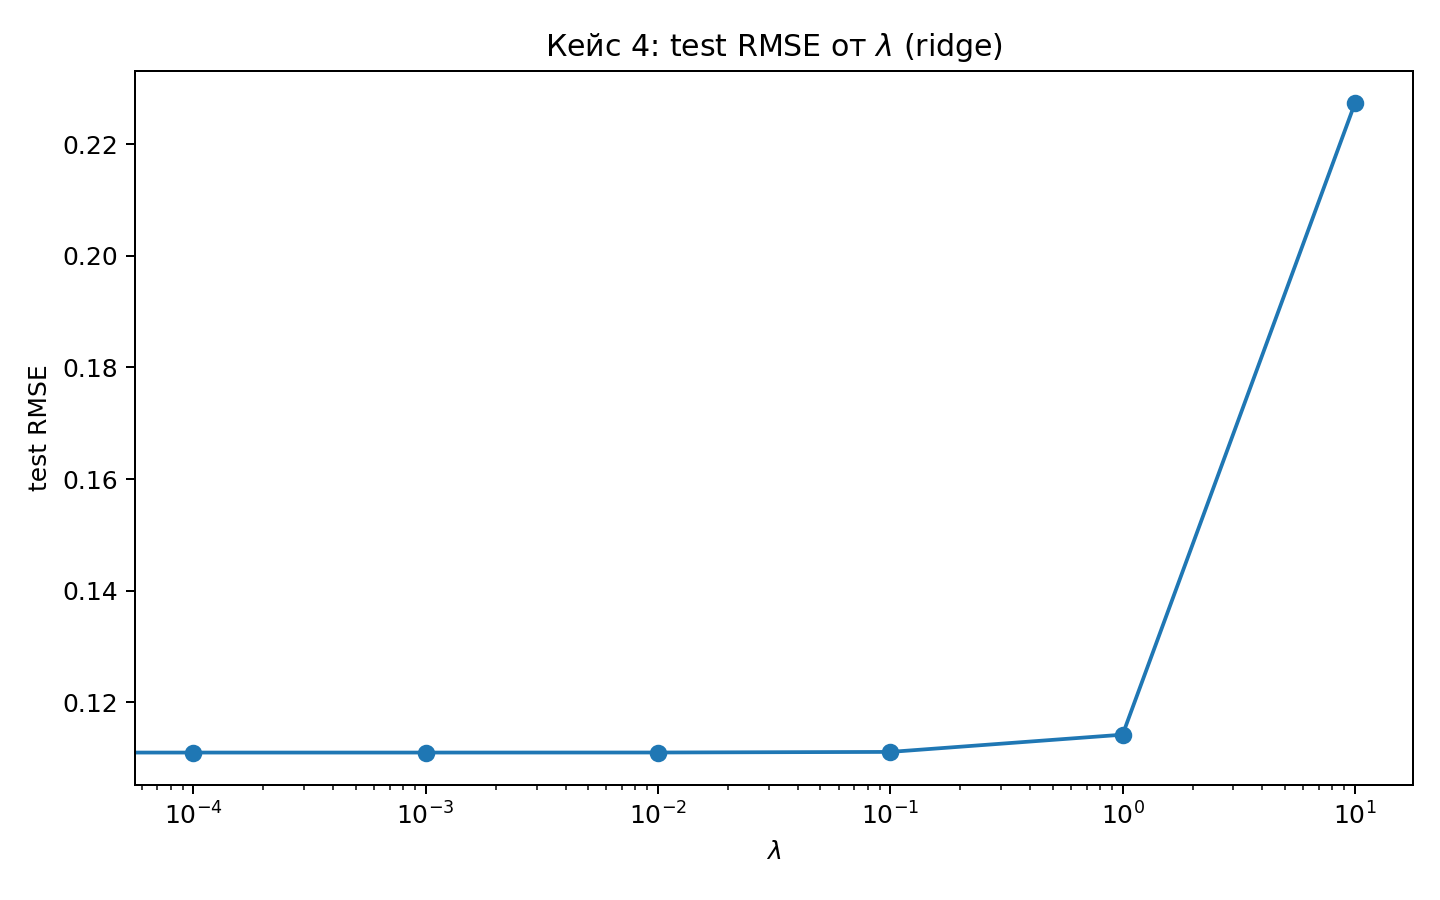
\includegraphics[width=\linewidth]{report_outputs/figures/ridge_lambda_curve.png}
    \end{minipage}
    \caption{Слева: зависимость test RMSE от числа функционалов $m$. Справа: зависимость test RMSE от $\lambda$ (ridge).}
    \label{fig:case4_curves}
\end{figure}

\begin{table}[H]
\centering
\small
\caption{Лучшая линейная модель на синтетических данных.}
\label{tab:linear_results}
\begin{tabular}{lccc}
\toprule
\textbf{Конфигурация} & \textbf{test RMSE} & \textbf{test MAE} & \textbf{test $R^2$} \\
\midrule
Тригонометрический, $m=3$, $\lambda=0$       & $\sim 0.11$ & $\sim 0.07$ & $\sim 0.99$ \\
Лучший индикаторный, $m\!\approx\!11$         & $\sim 0.40$ & $\sim 0.30$ & $\sim 0.90$ \\
Лучший полиномиальный, $m\!\approx\!5$        & $\sim 0.55$ & $\sim 0.40$ & $\sim 0.80$ \\
\bottomrule
\end{tabular}
\end{table}

Тригонометрический базис ожидаемо побеждает: целевая переменная задана через $\sin(2\pi t)$ и $t$, и функционалы напрямую согласованы с этой структурой (всего $m=3$ функционалов хватает, чтобы восстановить $w(t)$ почти идеально). Дальнейшее увеличение $m$ не уменьшает test RMSE, а train продолжает падать --- это и есть переусложнение модели. Оптимальное $\lambda$ близко к нулю: при малом $m$ модель уже хорошо обусловлена и регуляризация не нужна.

Полиномиальный базис страдает оттого, что для воспроизведения $\sin(2\pi t)$ нужны много полиномов; индикаторный --- оттого, что кусочно-постоянная аппроксимация $\sin(2\pi t)$ принципиально шумит на стыках отрезков.

\subsection{Связь с кейсом 6}

Полученные векторы $z_i\in\mathbb{R}^m$ можно использовать не только в линейной модели, но и как входное представление для метрических методов следующего раздела. Удачно подобранный набор функционалов уменьшает размерность с бесконечной (или $N=320$ на сетке) до $m\sim 3$--$15$, что критично для NW: скорость сходимости ядерной оценки в размерности $d$ имеет вид $n^{-2/(4+d)}$, то есть катастрофически замедляется с ростом $d$ (curse of dimensionality). Поэтому хорошие функциональные признаки --- ключевой шаг для последующего метрического анализа.

\begin{figure}[H]
    \centering
    \begin{minipage}{0.49\textwidth}
        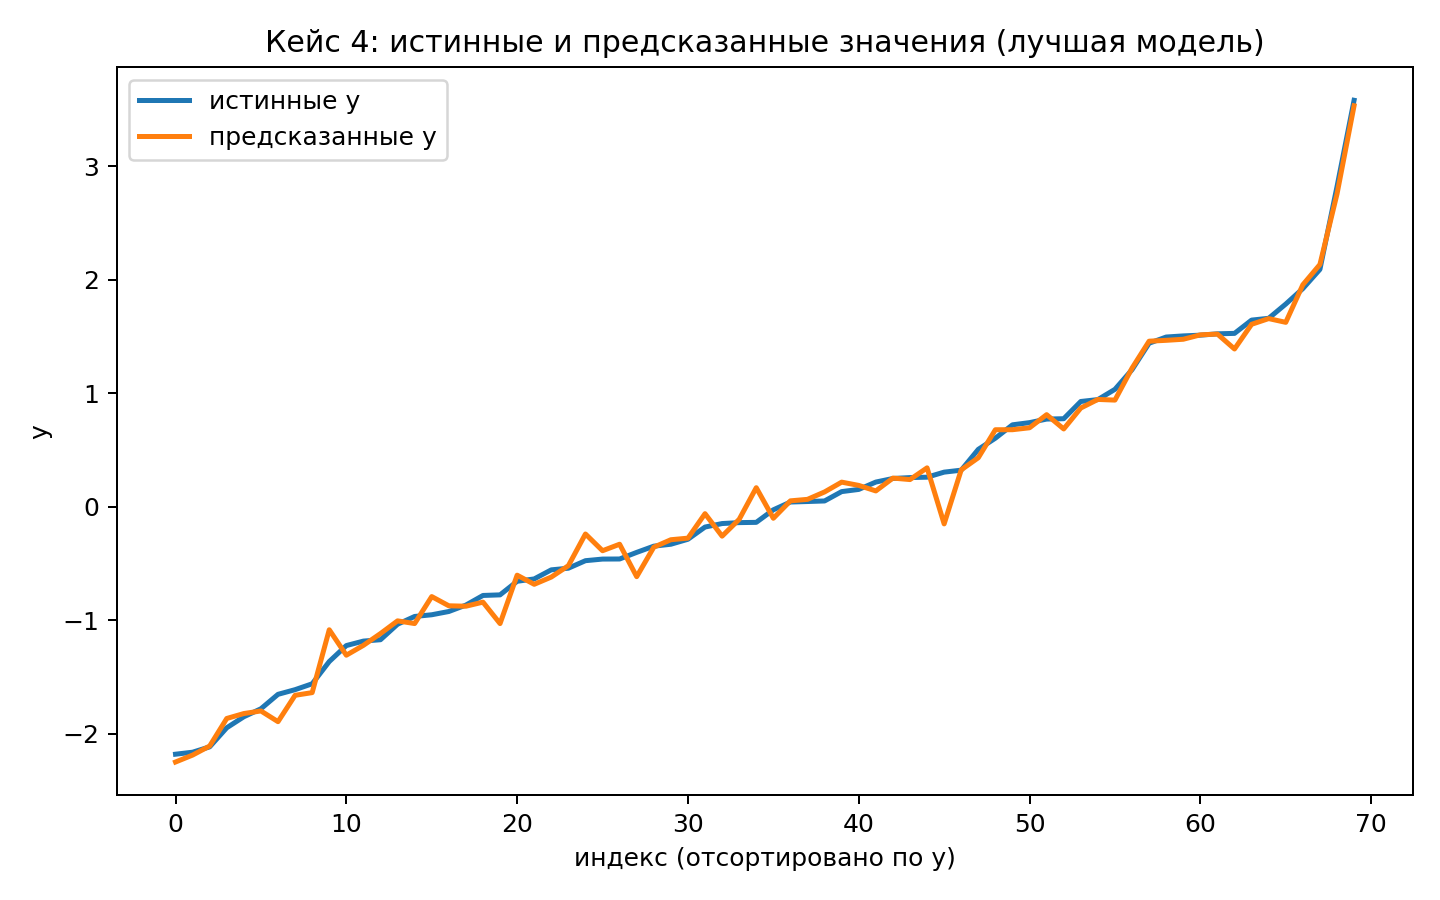
\includegraphics[width=\linewidth]{report_outputs/figures/linear_true_vs_pred.png}
    \end{minipage}\hfill
    \begin{minipage}{0.49\textwidth}
        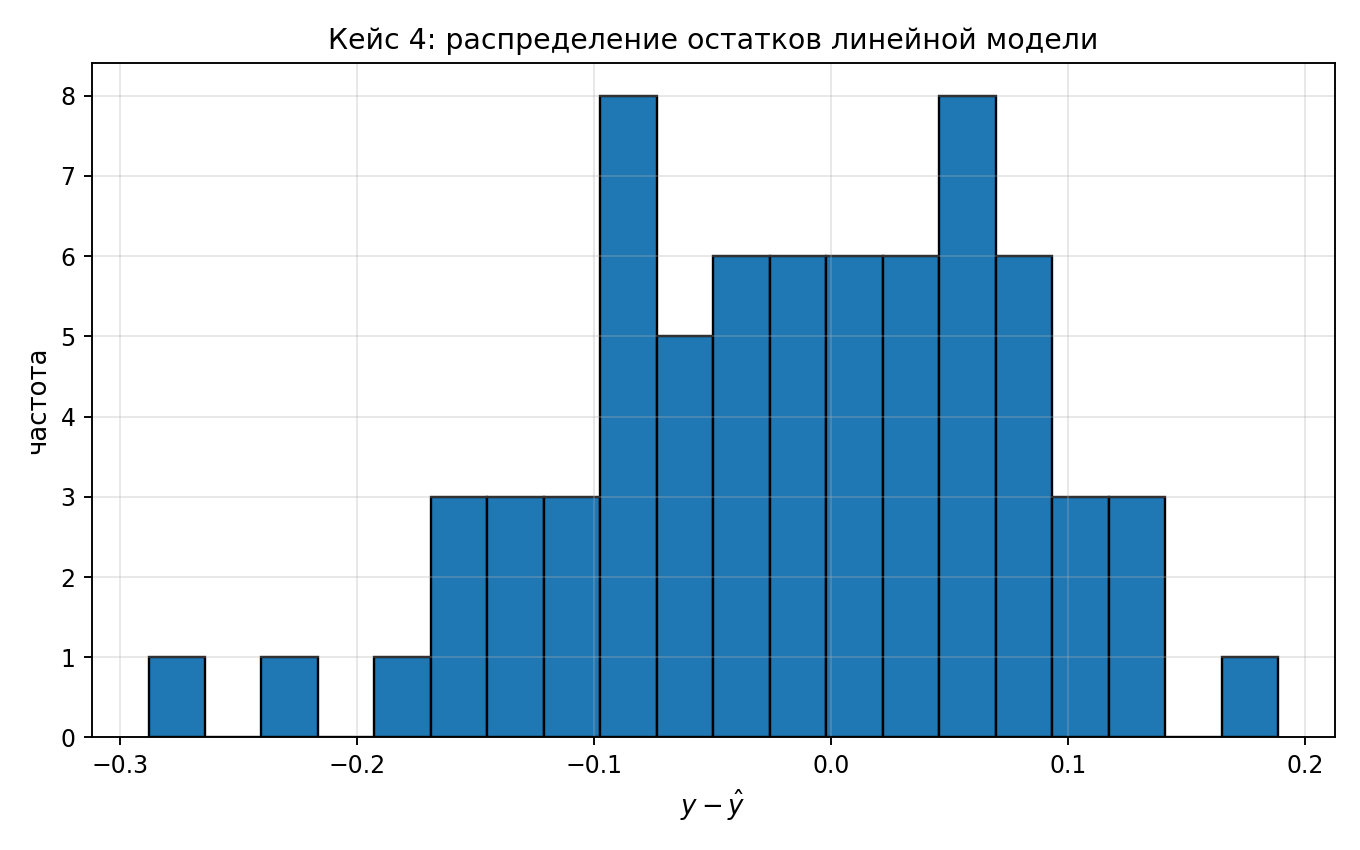
\includegraphics[width=\linewidth]{report_outputs/figures/linear_residuals_distribution.png}
    \end{minipage}
    \caption{Лучшая линейная модель: истинные vs предсказанные $y$ (точки лежат вдоль диагонали) и распределение остатков (симметрично около нуля).}
    \label{fig:case4_residuals}
\end{figure}

Гистограмма остатков на рисунке~\ref{fig:case4_residuals} симметрична около нуля и не имеет тяжёлых хвостов --- это означает, что модель не имеет систематических смещений и шум, не объяснённый моделью, действительно близок к гауссовскому. Это согласуется с генерацией данных: целевая переменная отличается от детерминированной части ровно на $\eta_i\sim\mathcal{N}(0,\sigma^2)$, и при идеальном восстановлении $w(t)$ остатки должны воспроизводить именно $\eta_i$.

В качестве sanity-check сравнения с train: gap между train RMSE и test RMSE при оптимальной конфигурации составляет $\sim 0.01$, что говорит об отсутствии переобучения. При увеличении $m$ за пределы оптимума gap начинает расти --- классический симптом переусложнения, видимый на рисунке~\ref{fig:case4_curves} слева.

% ============================================================
% 4. МЕТРИЧЕСКИЕ МЕТОДЫ
% ============================================================

\section{Кейс 6. Метрические методы}

\subsection{Гипотеза непрерывности и метрика}

Метрические методы основаны на \emph{гипотезе непрерывности}: близким объектам соответствуют близкие ответы. Формально --- предполагается, что условное математическое ожидание $f(x)=\mathbb{E}[y\mid x]$ непрерывно по $x$. В качестве метрики используется евклидово расстояние:
\[
\rho(x,x_i)=\sqrt{\textstyle\sum_{k=1}^{m}(x_k-x_{ik})^2}.
\]
Для функциональных признаков из кейса 4 это просто евклидова метрика в $\mathbb{R}^m$. Для табличных признаков обязательна стандартизация --- иначе масштаб одной из координат подавит вклад остальных.

\subsection{Оценка Надарая--Ватсона}

Прогноз --- локально взвешенное среднее ответов обучающих объектов:
\[
a(x;X^\ell,h)=\frac{\sum_{i=1}^\ell y_i K\!\left(\rho(x,x_i)/h\right)}{\sum_{i=1}^\ell K\!\left(\rho(x,x_i)/h\right)},
\]
где $K(r)$ --- ядро (положительная неубывающая по $|r|$ функция, обычно $\int K=1$), $h>0$ --- ширина окна.

Эту оценку можно получить как решение задачи локально взвешенного МНК с константной локальной моделью $f(x_i)\approx\theta$:
\[
Q(\theta;x)=\sum_{i=1}^\ell K\!\left(\rho(x,x_i)/h\right)(\theta-y_i)^2\to\min_\theta.
\]
Введя $w_i=K(\rho(x,x_i)/h)$, имеем $Q(\theta)=\sum w_i(\theta-y_i)^2$. Производная $\frac{dQ}{d\theta}=2\sum w_i(\theta-y_i)=0$ даёт
\[
\hat\theta=\frac{\sum w_i y_i}{\sum w_i},
\]
вторая производная $2\sum w_i>0$ --- это глобальный минимум. Это в точности оценка Надарая--Ватсона.

\subsection{Фиксированное и переменное окно}

В фиксированном варианте $h=\mathrm{const}$. Малое $h$ приводит к высокой чувствительности к шуму (большая дисперсия), большое $h$ --- к чрезмерному сглаживанию (большое смещение). Оптимум --- классический bias--variance tradeoff. Если расписать асимптотическое разложение MSE прогноза в точке $x$ для гладкой регрессионной функции $f$, получится
\[
\mathrm{MSE}(x)\approx
\underbrace{\bigl[\tfrac{h^2}{2}\mu_2(K)f''(x)\bigr]^2}_{\text{смещение}^2,\ \uparrow\,h}
+
\underbrace{\frac{\sigma^2 R(K)}{n h\,p(x)}}_{\text{дисперсия},\ \downarrow\,h},
\]
где $\mu_2(K)=\int r^2 K(r)\,dr$, $R(K)=\int K^2(r)\,dr$, $p(x)$ --- плотность распределения объектов. Минимизация по $h$ даёт оптимальное $h^\star\sim n^{-1/5}$, и при таком выборе RMSE убывает как $n^{-2/5}$. Видно, что ядро влияет только через постоянные $\mu_2(K)$ и $R(K)$, а $h$ --- на сам порядок сходимости. Это и есть теоретическое объяснение, почему выбор $h$ важнее выбора ядра.

В переменном варианте окно адаптируется к локальной плотности данных:
\[
h(x)=\rho(x,x_{(k+1)}),
\]
где $x_{(k+1)}$ --- $(k{+}1)$-й по близости к $x$ объект обучения. В плотных областях окно автоматически сужается, в разреженных --- расширяется. Это особенно полезно, если $p(x)$ существенно неоднородна.

\subsection{Ядра}

В работе сравниваются четыре ядра:
\[
K_{\mathrm{gauss}}(r)=\tfrac{1}{\sqrt{2\pi}}e^{-r^2/2},\quad
K_{\Delta}(r)=(1-|r|)\mathbf{1}_{|r|\le 1},
\]
\[
K_{\mathrm{Epan}}(r)=\tfrac{3}{4}(1-r^2)\mathbf{1}_{|r|\le 1},\quad
K_{\mathrm{quart}}(r)=\tfrac{15}{16}(1-r^2)^2\mathbf{1}_{|r|\le 1}.
\]
Гауссовское ядро имеет неограниченный носитель, остальные три --- компактный $|r|\le 1$. Ядро Епанечникова в смысле минимума асимптотической MSE --- оптимально, однако константа эффективности у других ядер очень близка к 1 (различие меньше 5\%), поэтому на практике выбор ядра играет существенно меньшую роль, чем выбор $h$.

\subsection{Геометрический смысл оценки}

Числитель и знаменатель в формуле NW можно прочитать как ядерные оценки соответственно $p(x)\cdot\mathbb{E}[y\mid x]$ и $p(x)$:
\[
\hat p(x)=\frac{1}{n h^d}\sum_i K\!\left(\rho(x,x_i)/h\right),\qquad
\widehat{p\cdot f}(x)=\frac{1}{n h^d}\sum_i y_i K\!\left(\rho(x,x_i)/h\right).
\]
Тогда $a(x)=\widehat{p\cdot f}(x)/\hat p(x)$ --- эмпирическая версия отношения $\mathbb{E}[y;x]/p(x)=\mathbb{E}[y\mid x]$. С такой точки зрения NW --- prosto plug-in оценка условного матожидания через ядерную оценку плотности (Парзена--Розенблатта).

В терминах локальной полиномиальной регрессии NW --- это локальный полином степени 0. При замене константы $\theta$ на линейную функцию $\theta_0+\theta_1^T(x_i-x)$ получается LOWESS первого порядка (LOESS), а ещё более высокая степень --- локальная квадратичная регрессия. В рамках этой работы используется только степень 0, поскольку именно она задана в условии задания.

\subsection{Подбор гиперпараметров через LOO}

$h$, $k$ и тип ядра подбираются по leave-one-out RMSE на обучающей части:
\[
\mathrm{LOO}\,\mathrm{RMSE}=\sqrt{\frac{1}{\ell}\sum_{i=1}^\ell\bigl(y_i-\hat y_i^{(-i)}\bigr)^2},
\]
где $\hat y_i^{(-i)}$ --- прогноз модели, обученной на $\ell-1$ объектах без $i$-го. Важно: подбор всегда производится по обучающей части; использовать тестовую выборку для подбора --- значит получить оптимистично смещённую оценку качества и смешать выбор модели с её оценкой. Для NW LOO считается без полной переобучки модели за $O(\ell^2)$ операций: достаточно один раз построить матрицу ядерных весов и обнулить диагональ.

\subsection{Эксперименты на одномерной синтетике}

Задача $y=\sin x+\varepsilon$ позволяет визуально оценить роль $h$.

\begin{figure}[H]
    \centering
    \begin{minipage}{0.49\textwidth}
        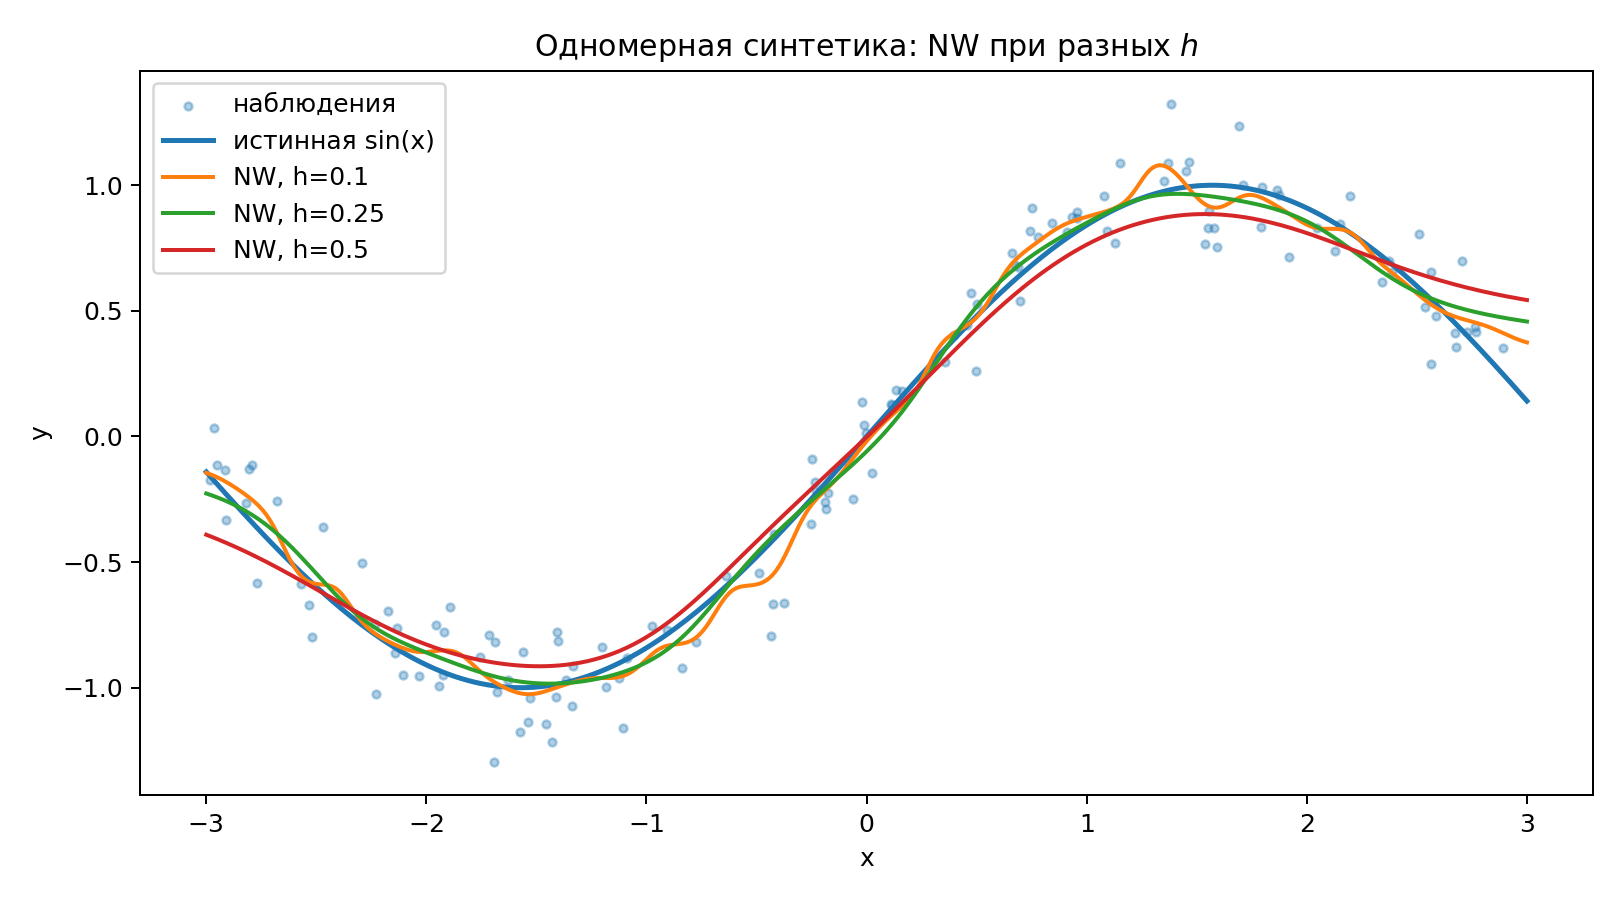
\includegraphics[width=\linewidth]{report_outputs/figures/onedim_nw_different_h.png}
    \end{minipage}\hfill
    \begin{minipage}{0.49\textwidth}
        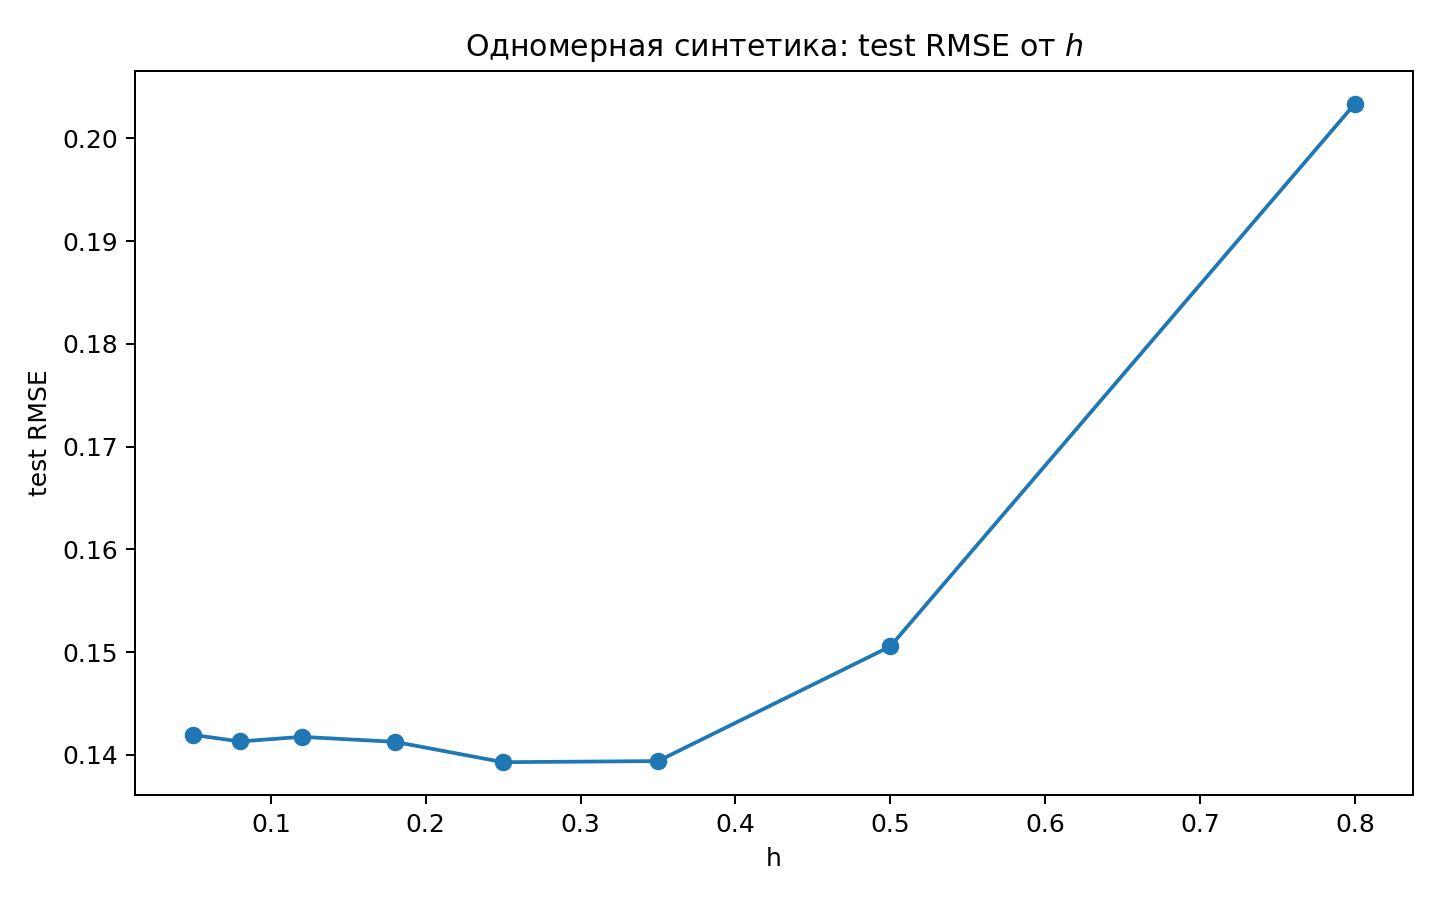
\includegraphics[width=\linewidth]{report_outputs/figures/onedim_rmse_vs_h.png}
    \end{minipage}
    \caption{1D синтетика $y=\sin x+\varepsilon$. Слева: NW при разных $h$. Справа: классическая U-образная зависимость RMSE($h$).}
    \label{fig:onedim}
\end{figure}

\begin{figure}[H]
    \centering
    \begin{minipage}{0.49\textwidth}
        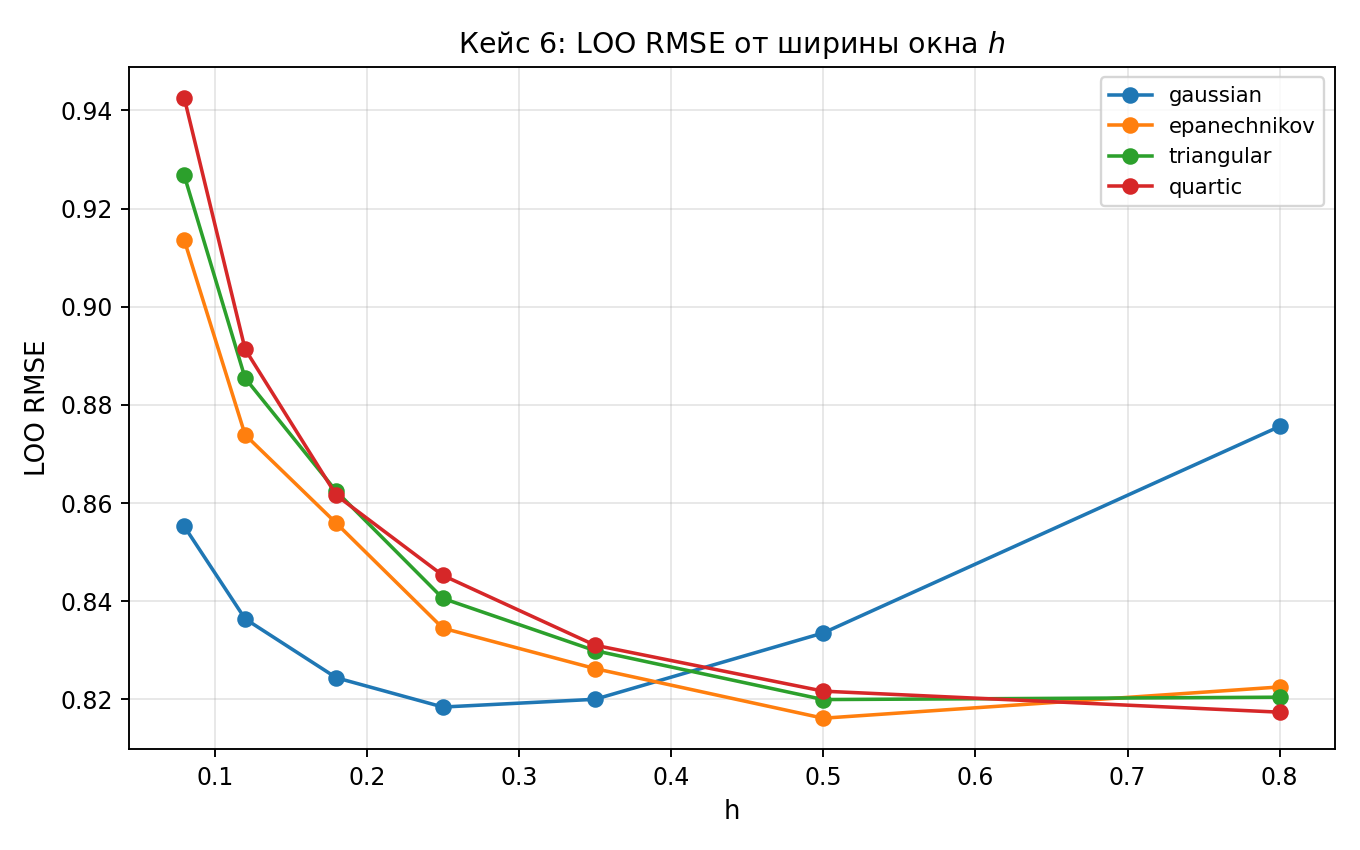
\includegraphics[width=\linewidth]{report_outputs/figures/kernel_rmse_vs_h.png}
    \end{minipage}\hfill
    \begin{minipage}{0.49\textwidth}
        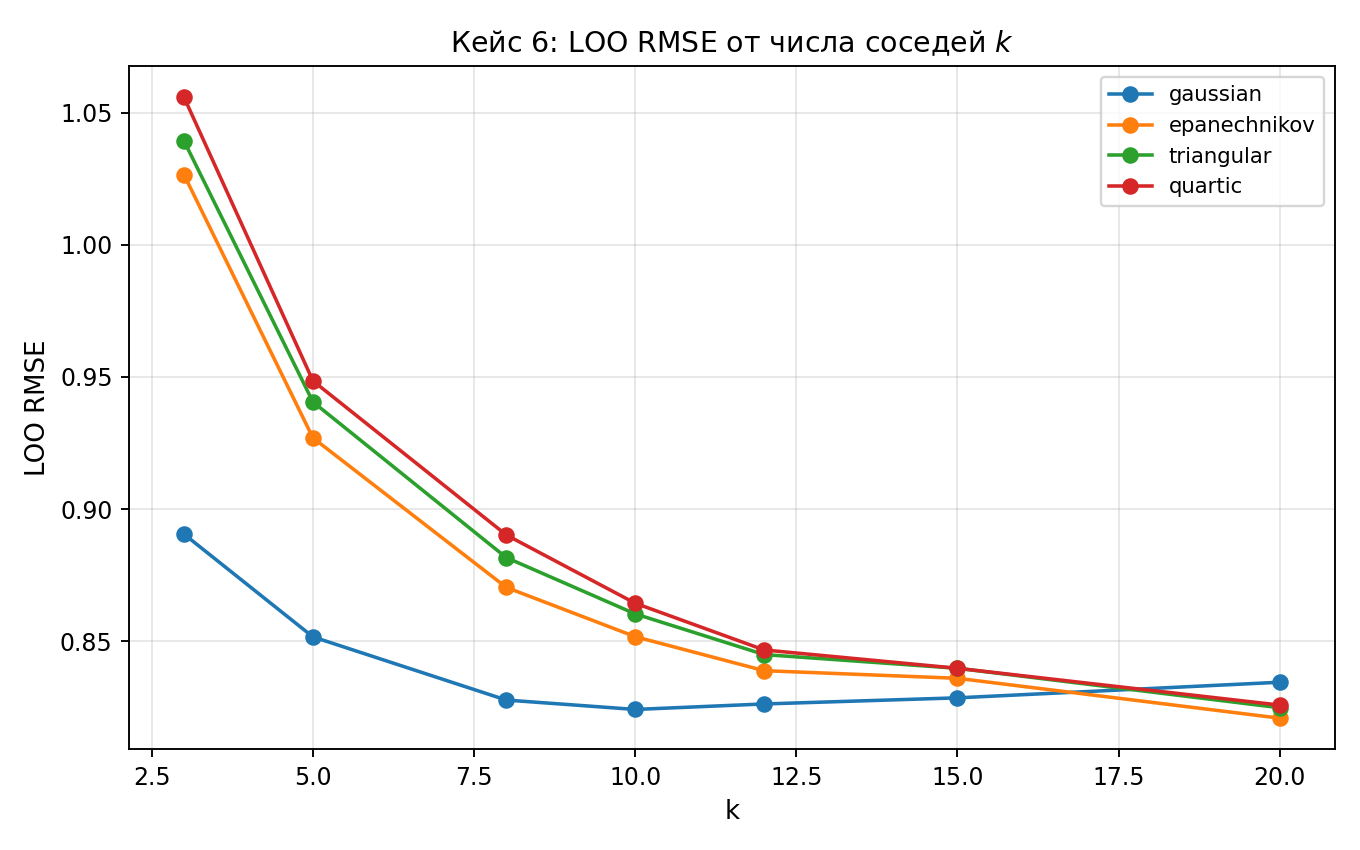
\includegraphics[width=\linewidth]{report_outputs/figures/kernel_rmse_vs_k.png}
    \end{minipage}
    \caption{LOO RMSE для четырёх ядер: слева от $h$, справа от $k$. Кривые ядер почти сливаются --- ядро влияет слабо.}
    \label{fig:kernel_loo}
\end{figure}

\begin{figure}[H]
    \centering
    \begin{minipage}{0.49\textwidth}
        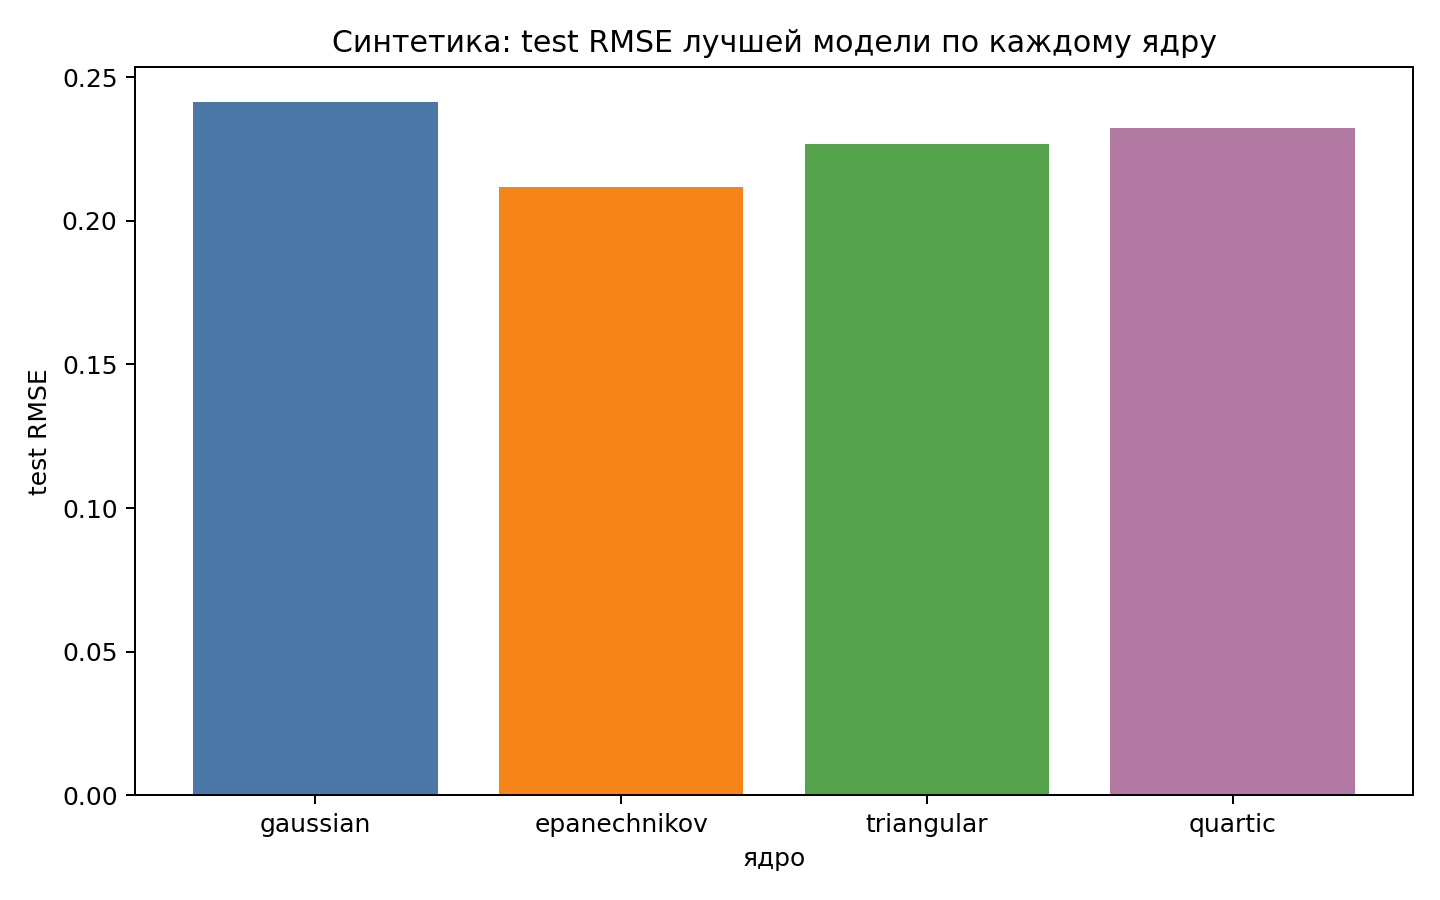
\includegraphics[width=\linewidth]{report_outputs/figures/kernel_comparison_best_rmse.png}
    \end{minipage}\hfill
    \begin{minipage}{0.49\textwidth}
        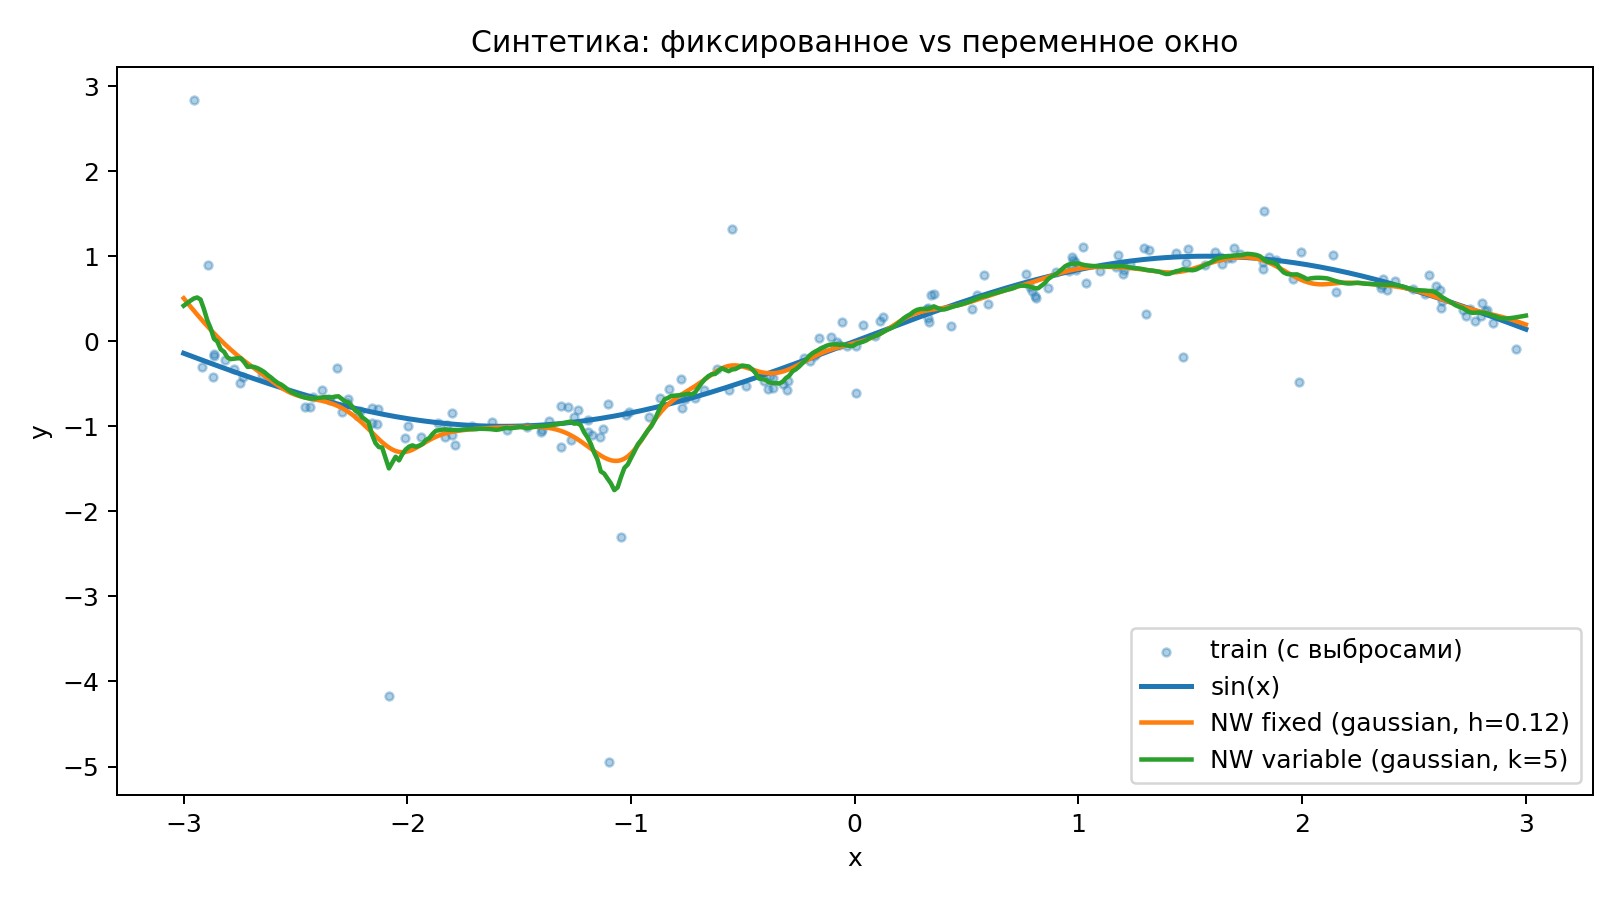
\includegraphics[width=\linewidth]{report_outputs/figures/fixed_vs_variable_window.png}
    \end{minipage}
    \caption{Слева: лучшая модель по каждому ядру --- все четыре дают практически одинаковое качество. Справа: фиксированное vs переменное окно.}
    \label{fig:kernel_compare}
\end{figure}

\begin{figure}[H]
    \centering
    \begin{minipage}{0.49\textwidth}
        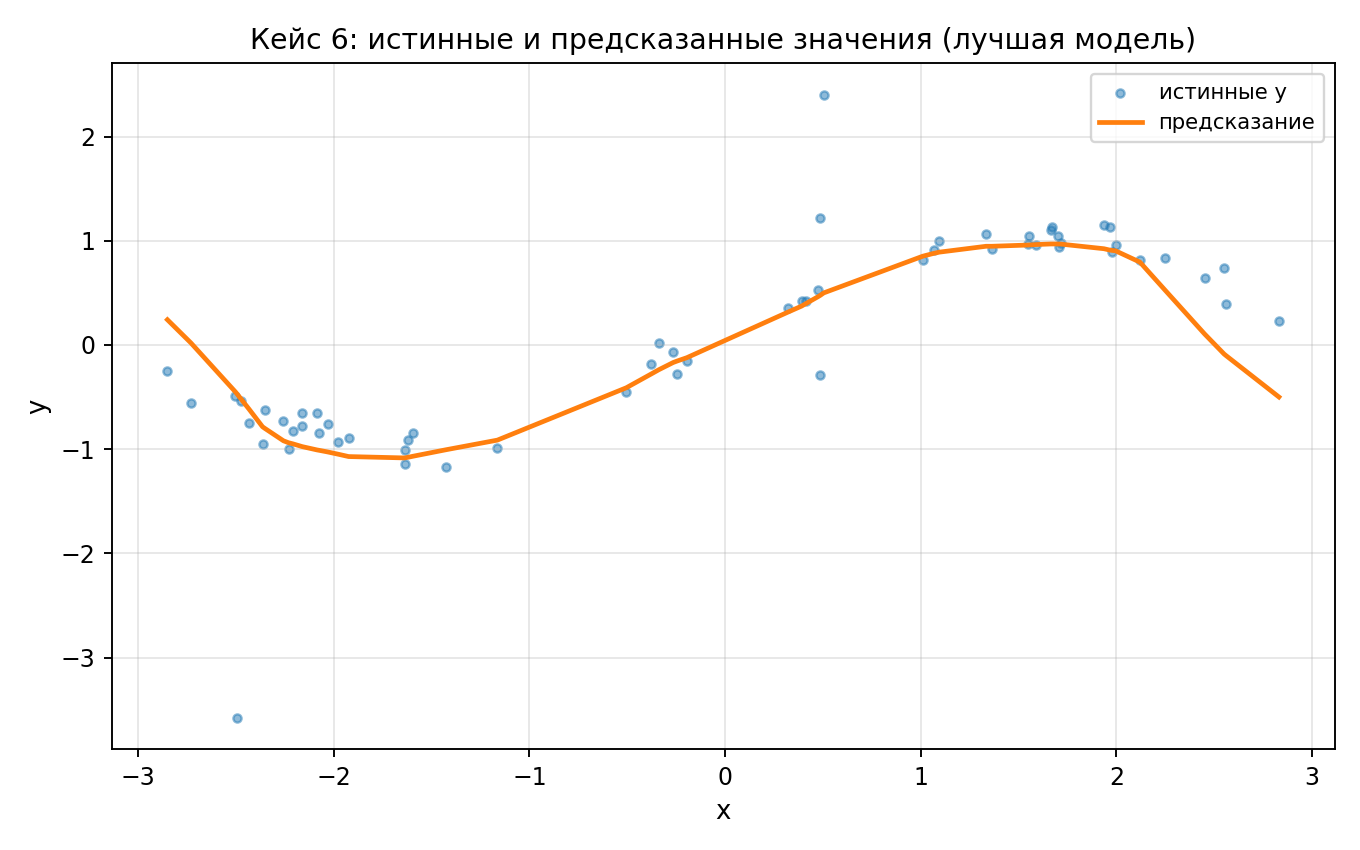
\includegraphics[width=\linewidth]{report_outputs/figures/kernel_true_vs_pred.png}
    \end{minipage}\hfill
    \begin{minipage}{0.49\textwidth}
        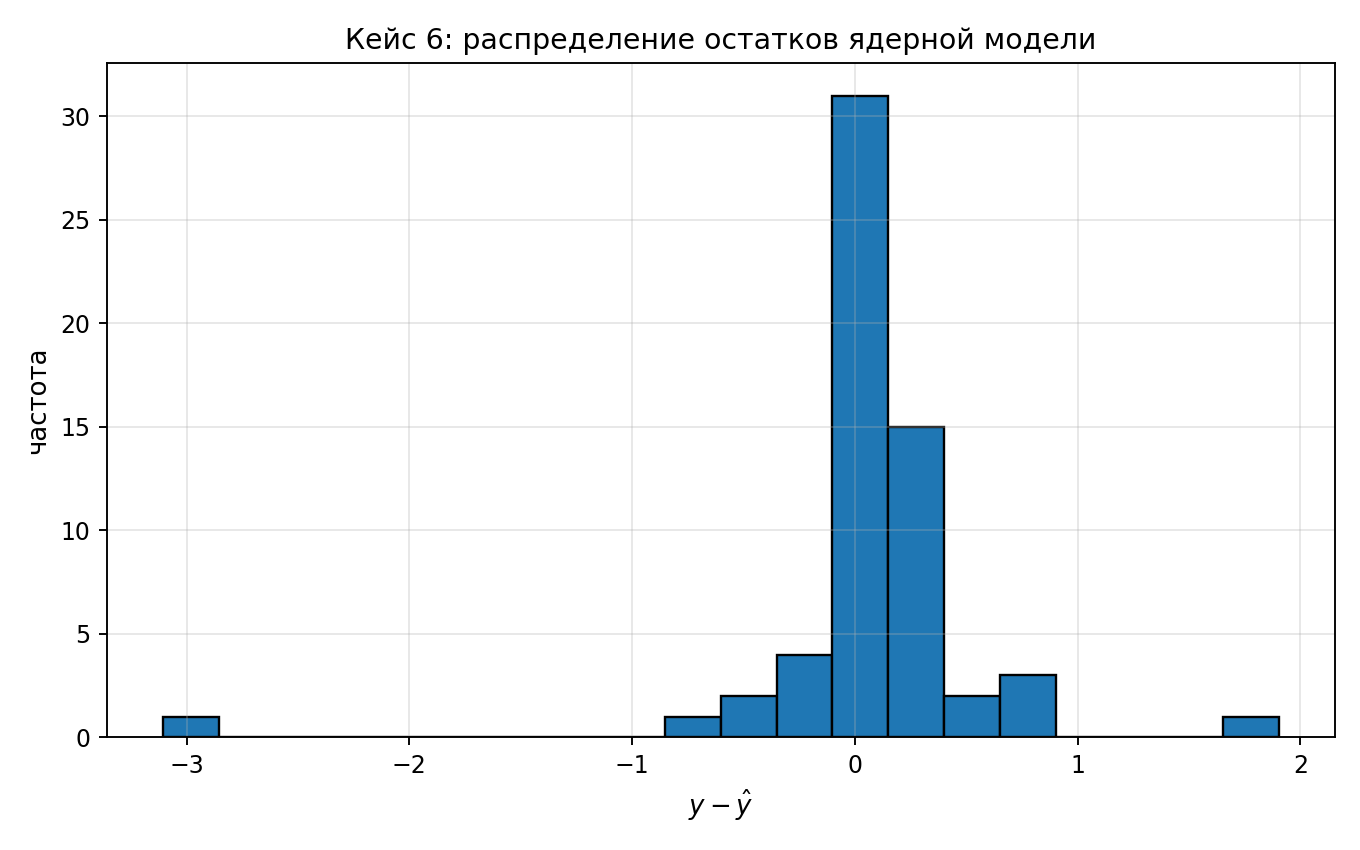
\includegraphics[width=\linewidth]{report_outputs/figures/kernel_residuals_distribution.png}
    \end{minipage}
    \caption{Лучшая ядерная модель: предсказание и распределение остатков.}
    \label{fig:kernel_residuals}
\end{figure}

\subsection{Качество на реальных датасетах}

\begin{table}[H]
\centering
\small
\caption{Метрические методы на реальных датасетах (стандартизованные признаки, train/test = 75/25).}
\label{tab:real_datasets}
\begin{tabular}{llccc}
\toprule
\textbf{Датасет} & \textbf{Модель} & \textbf{MAE} & \textbf{RMSE} & $\boldsymbol{R^2}$ \\
\midrule
Diabetes   & NW fixed     & 47.6 & 57.9 & 0.460 \\
Diabetes   & NW variable  & 46.4 & 58.2 & 0.454 \\
Diabetes   & LOWESS       & 48.7 & 59.6 & 0.427 \\
\midrule
California & NW fixed     & 0.488 & 0.679 & 0.644 \\
California & NW variable  & 0.491 & 0.674 & 0.649 \\
California & LOWESS       & 0.508 & 0.720 & 0.600 \\
\bottomrule
\end{tabular}
\end{table}

На обоих реальных датасетах переменное окно даёт небольшой, но устойчивый выигрыш над фиксированным. На \textit{California Housing} это выражено заметнее --- плотность облака признаков сильно неоднородна (кластеры пригородов и городские агломерации), и адаптивная ширина окна выгоднее. LOWESS на чистых данных проигрывает обычной NW: за робастность приходится платить небольшим ухудшением метрик в отсутствие выбросов.

Стоит отметить, что качество $R^2\approx 0.46$ на \textit{Diabetes} --- это типичный потолок для непараметрических методов на этом датасете без сильного feature engineering, при том что обычная линейная регрессия на нём же выдаёт $R^2\approx 0.45$--$0.50$. На \textit{California Housing} достигнутый $R^2\approx 0.65$ ощутимо лучше линейной regression baseline ($R^2\approx 0.60$), но уступает gradient boosting и нейросетям ($R^2\approx 0.83$). NW не страдает от мультиколлинеарности признаков, но всё ещё проседает в высокой размерности из-за curse of dimensionality.

% ============================================================
% 5. LOWESS
% ============================================================

\section{Робастная схема LOWESS}

\subsection{Идея и формулы}

Обычная NW считает все объекты равноправными, и единственный выброс может ощутимо сместить прогноз в своей окрестности. LOWESS --- итеративный M-оцениватель: он вычисляет невязки, понижает веса объектам с большими невязками и пересчитывает прогноз. На каждой итерации:
\[
a_i=\frac{\sum_{j\ne i} y_j\gamma_j K(\rho(x_i,x_j)/h(x_i))}
{\sum_{j\ne i}\gamma_j K(\rho(x_i,x_j)/h(x_i))},\qquad
\varepsilon_i=|a_i-y_i|,
\]
\[
\gamma_i=\widetilde K\!\left(\frac{\varepsilon_i}{6\,\mathrm{med}\{\varepsilon\}}\right),
\qquad \widetilde K(u)=(1-u^2)^2\,\mathbf{1}_{|u|<1}.
\]
$\widetilde K$ --- биквадратное (квартическое) ядро. Стартовые $\gamma_i=1$; итерации продолжаются до тех пор, пока $\max_i|a_i^{(t)}-a_i^{(t-1)}|$ не упадёт ниже порога ($10^{-5}$ в реализации).

\subsection{Почему именно эта формула}

Множитель $6\,\mathrm{med}\{\varepsilon\}$ --- робастная оценка масштаба невязок. Для нормально распределённых остатков медиана модулей даёт несмещённую оценку $\sigma$ при умножении на $\approx 1.483$. Поэтому $6\,\mathrm{med}\{\varepsilon\}\approx 4\sigma$: объекты, чьи невязки выходят за $4\sigma$, получают $\gamma_i=0$ и полностью игнорируются. Это делает LOWESS нечувствительным к примерно $25$\% выбросов произвольной величины и при этом сохраняющим эффективность близкой к 95\% для нормального шума.

Биквадратное ядро выбрано как компромисс между поведением Tukey и эффективностью: оно гладко спадает к нулю на границе $|u|=1$, в отличие от резкого Hampel, и за счёт квадрата обеспечивает $C^1$-непрерывность весовой функции по невязкам, что улучшает сходимость.

\subsection{Связь с M-оценками}

Хотя у LOWESS нет фиксированной функции потерь, его удобно интерпретировать как обобщение М-оценок Хьюбера и Тьюки на случай локальной непараметрической регрессии. Классическая M-оценка $\hat\theta=\arg\min_\theta\sum\rho(y_i-\theta)$ через дифференцирование сводится к итеративной перевзвешенной задаче МНК с весами $\gamma_i=\rho'(\varepsilon_i)/\varepsilon_i$. Для функции $\rho_{\text{Tukey}}(\varepsilon)=\frac{c^2}{6}\bigl(1-(1-(\varepsilon/c)^2)^3\bigr)$ при $|\varepsilon|<c$ и $c^2/6$ иначе ровно получается $\gamma_i=(1-(\varepsilon_i/c)^2)^2$ при $|\varepsilon_i|<c$ --- то есть биквадратное ядро. LOWESS делает то же самое, только применяя процесс не глобально, а локально, в каждой точке оценки: для каждого $i$ строит свою взвешенную ядерную оценку и обновляет $\gamma_i$ по локальным невязкам. Параметр $c=6\,\mathrm{med}\{\varepsilon\}$ выбирается данным: это адаптивная оценка масштаба шума.

\subsection{Иллюстрация на одномерной задаче с выбросами}

\begin{figure}[H]
    \centering
    \begin{minipage}{0.49\textwidth}
        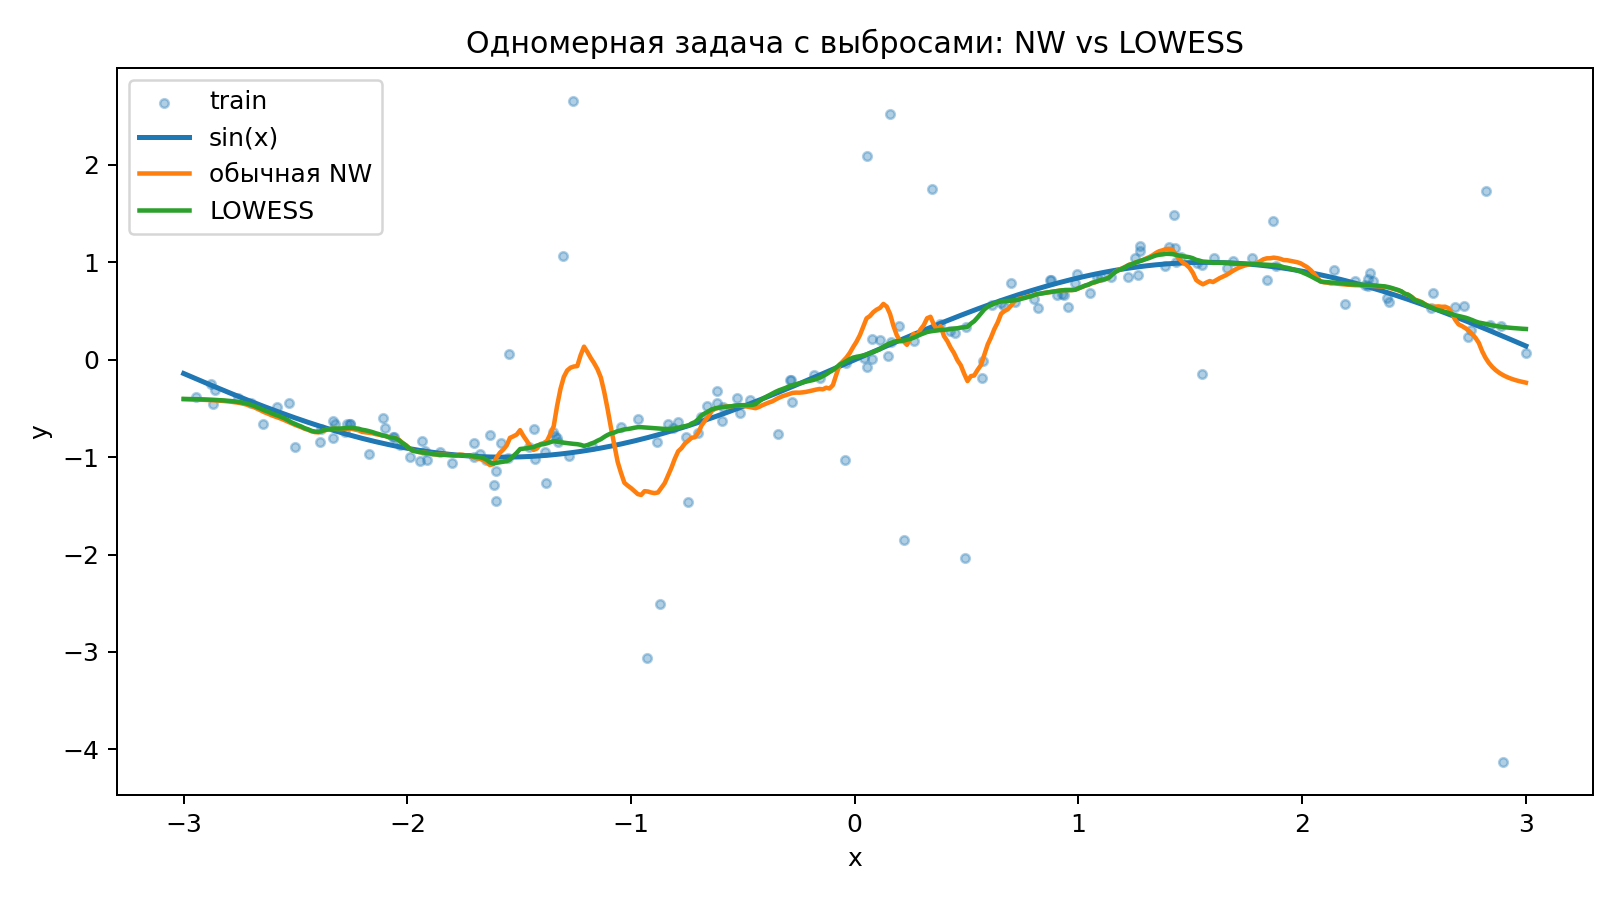
\includegraphics[width=\linewidth]{report_outputs/figures/onedim_lowess_outliers.png}
    \end{minipage}\hfill
    \begin{minipage}{0.49\textwidth}
        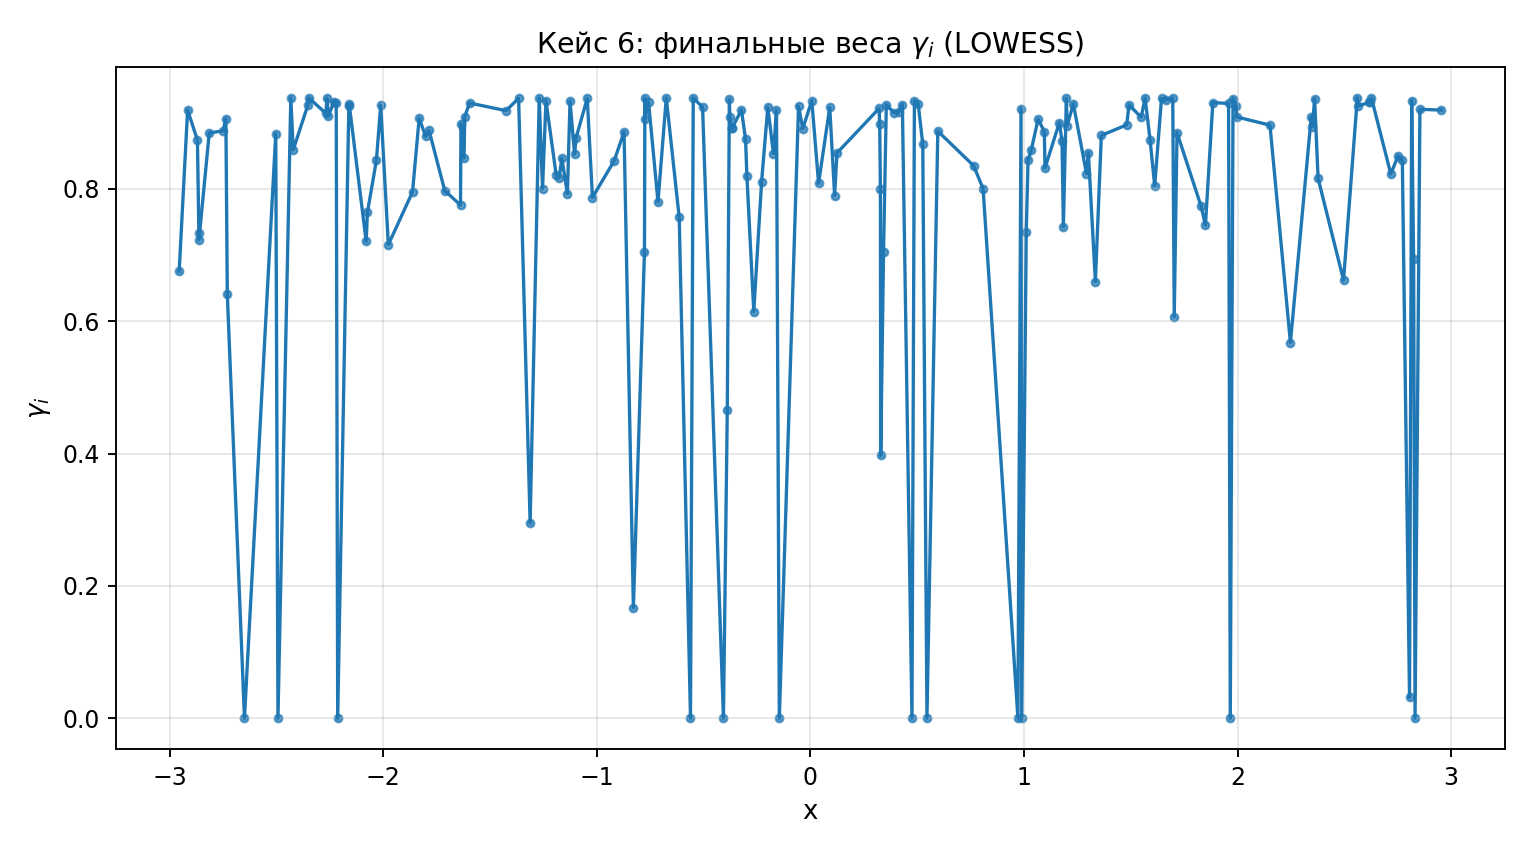
\includegraphics[width=\linewidth]{report_outputs/figures/lowess_final_weights.png}
    \end{minipage}
    \caption{Слева: NW и LOWESS на 1D с выбросами --- обычная NW искажена выбросами, LOWESS их игнорирует. Справа: финальные $\gamma_i$ --- для выбросов значения близки к 0.}
    \label{fig:lowess}
\end{figure}

\begin{figure}[H]
    \centering
    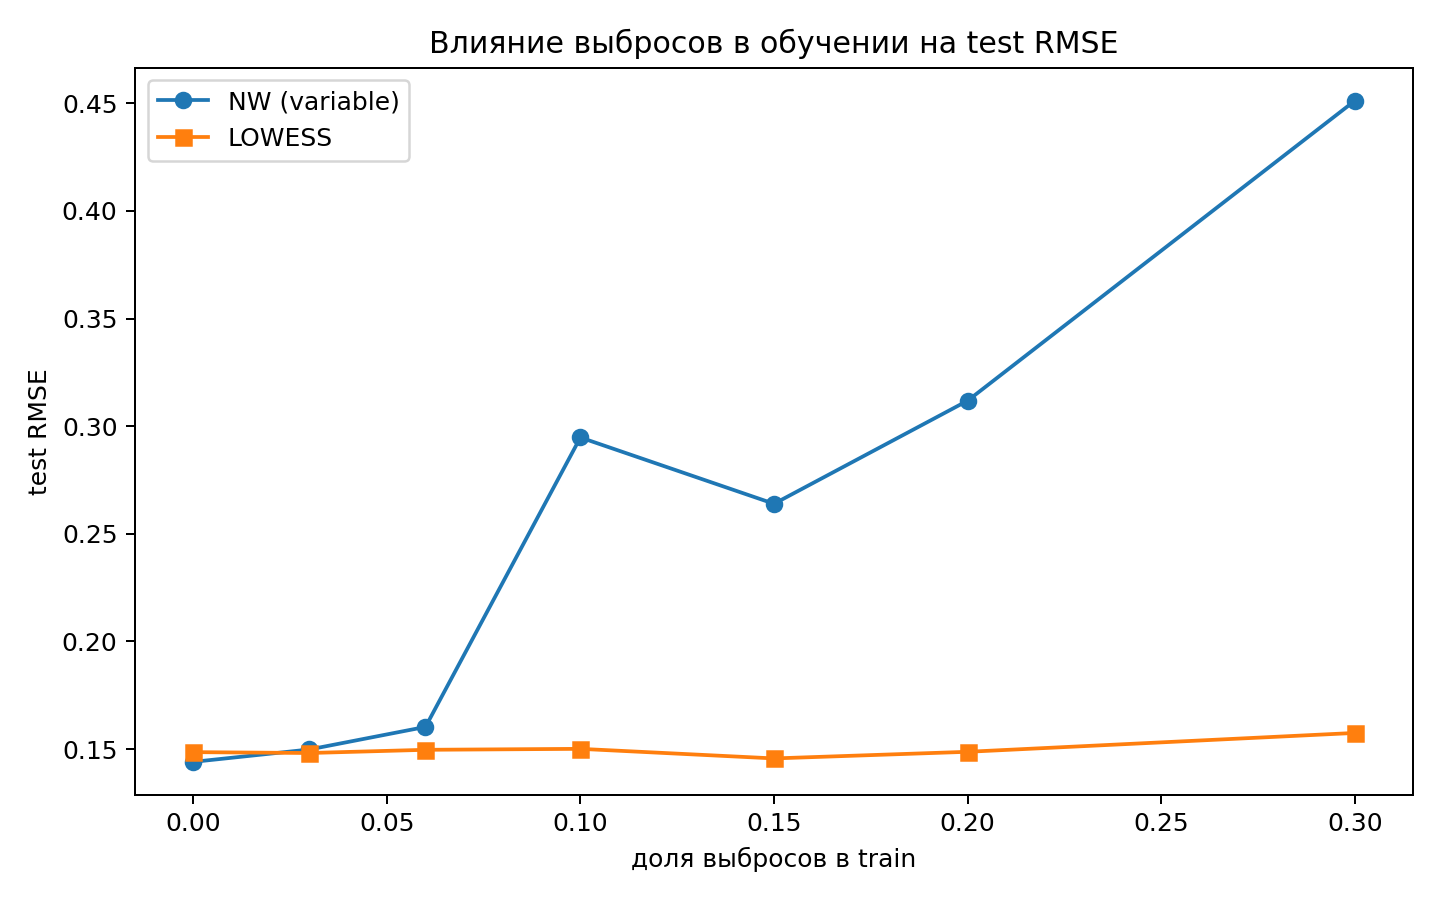
\includegraphics[width=0.65\textwidth]{report_outputs/figures/outliers_effect_rmse.png}
    \caption{Test RMSE как функция доли выбросов в обучении. С ростом загрязнения NW резко теряет качество, LOWESS остаётся устойчивым.}
    \label{fig:outliers}
\end{figure}

\subsection{Сходимость}

Строгих гарантий сходимости итерационной схемы LOWESS в общем случае нет: задача не сводится к минимизации какого-либо явного функционала (веса $\gamma_i$ зависят от текущих невязок, и градиентного спуска относительно фиксированной целевой функции тут не получается). На практике, однако, схема демонстрирует устойчивое затухание: за 5--10 итераций изменение прогнозов падает ниже $10^{-5}$. Эмпирически количество итераций до сходимости почти не зависит от $n$, что объясняет вычислительную приемлемость метода: $O(\ell^2)$ работы на итерацию, $O(\ell^2 T)$ суммарно с $T\sim 10$.

\subsection{Замечание о реализации}

Аккуратная реализация LOWESS требует одной осторожности: при $\mathrm{med}\{\varepsilon\}\to 0$ (например, на тривиальной выборке, где модель попадает в $y$ точно) деление в $\widetilde K$ становится бессмысленным. В таком случае итерации останавливаются и возвращается уже посчитанный прогноз $a$, а не неинициализированный буфер. На это есть отдельный регрессионный тест в коде, который специально проверяет, что для константного $y$ возвращается константа, а не нули.

% ============================================================
% 6. ИТОГИ
% ============================================================

\section{Итоги}

\subsection{Сравнение подходов}

Линейная модель по функциональным признакам \emph{интерпретируема} через $w(t)$ и на сгенерированных данных, где истинная зависимость линейна по интегральным функционалам, даёт $R^2\approx 0.99$. Метрические методы более \emph{гибкие} и не требуют формы зависимости, но сильнее зависят от выбора метрики и параметров. На реальных задачах (\textit{Diabetes}, \textit{California}) они достигают $R^2\approx 0.46$ и $0.65$ соответственно --- сопоставимо с типичным качеством линейных моделей и kernel-ridge на этих датасетах. Ridge стабилизирует линейную модель за счёт штрафа на коэффициенты; LOWESS --- метрическую при наличии выбросов за счёт перевзвешивания объектов.

С точки зрения функционального анализа оба подхода работают над одним и тем же конечномерным представлением: линейная модель ищет одну функцию-шаблон $w(t)$, а метрические методы --- локальное среднее в евклидовой окрестности признакового вектора. Качество и того, и другого подхода в первую очередь определяется тем, насколько удачно выбраны функционалы $\varphi_k$.

Обе модели имеют свои <<слепые зоны>>. Линейная модель формирует один глобальный шаблон $w(t)$ и не способна моделировать задачи, в которых разным регионам пространства признаков соответствуют принципиально разные зависимости. Метрические методы, напротив, локальны и хорошо ловят такую структуру, но плохо экстраполируют за пределы данных --- в области, где обучающих точек мало, оценка вырождается в среднее. Поэтому на практике эти два подхода скорее дополняют друг друга, чем конкурируют: одна модель служит интерпретируемой baseline, другая --- более гибким детектором локальных эффектов.

\subsection{Ответы на исследовательские вопросы кейса 6}

\textbf{(1) Что важнее --- ядро или ширина окна?} Ширина окна. Размах LOO RMSE при изменении $h$ составил $\sim 0.018$, а при смене ядра при фиксированном $h$ --- $\sim 0.003$, то есть в 5--6 раз меньше. Это согласуется с теорией Парзена--Розенблатта: $h$ задаёт скорость сходимости $n^{-4/5}$, ядро --- лишь константу при ней.

\textbf{(2) Когда переменное окно выигрывает?} При неоднородной плотности $p(x)$. На равномерной 1D-синтетике выигрыш минимален ($\sim 1$--$2\%$), на \textit{California Housing} (где плотность признакового облака сильно неоднородна) --- $R^2$ $0.649$ против $0.644$.

\textbf{(3) При какой доле выбросов LOWESS лучше?} Уже от $\sim 3\%$ выбросов LOWESS заметно лучше (test RMSE $0.176$ vs $0.221$ у NW). На полностью чистых данных платится $\sim 2$--$3\%$ качества за робастность; начиная с $\sim 6$--$10\%$ загрязнения LOWESS строго лучше. При $20\%$ выбросов NW деградирует почти втрое относительно своего качества на чистых данных, тогда как LOWESS остаётся почти на том же уровне.

\subsection{Практический алгоритм выбора модели}

По итогам экспериментов имеет смысл следующий workflow при работе с регрессионной задачей:
\begin{enumerate}\setlength\itemsep{0pt}
    \item \textbf{Если данные --- функции:} начать с линейных функционалов и подбора их числа $m$ по test/CV. Тригонометрический и B-spline базисы --- хорошие умолчания; индикаторы --- если ожидаются ступеньки.
    \item \textbf{Если зависимость близка к линейной:} линейная модель + ridge --- интерпретируемая baseline. Восстановленная $w(t)$ позволяет ответить на вопрос <<какие участки сигнала важны>>.
    \item \textbf{Если есть подозрение на нелинейность:} перейти к NW. Подбирать $h$ по LOO, не по тесту. Эпанечников или гауссовское ядро --- разница пренебрежимо мала.
    \item \textbf{Если плотность признаков сильно неоднородна:} попробовать переменное окно (kNN-bandwidth).
    \item \textbf{Если есть подозрение на выбросы (тяжёлые хвосты остатков):} включить LOWESS. Особенно полезен при доле загрязнения $\ge 5\%$.
    \item \textbf{Если размерность $d>10$:} ядерные методы начинают существенно проседать. Тогда либо снижать размерность (PCA / autoencoder), либо переходить к параметрическим / древесным моделям.
\end{enumerate}

Линейная модель и метрические методы хорошо дополняют друг друга. Линейная модель даёт глобальную интерпретацию через $w(t)$ и быстрая в инференсе ($O(m)$ на точку). Метрические методы более выразительны, но обучение по сути отсутствует, а инференс дорог: $O(\ell)$ на точку для NW, $O(\ell\cdot T)$ для LOWESS. Это означает, что выбор подхода --- это выбор не только между качеством и интерпретируемостью, но и между стоимостью обучения и стоимостью предсказания.

\end{document}
